\begin{dang}{Cực trị hàm hợp, hàm chứa trị tuyệt đối}
    \begin{itemize}
        \item Các phép biến đổi đồ thị
        \begin{itemize}
            \item Đồ thị hàm $y=f(x+a)$ vẽ bằng cách dời đồ thị $y=f(x)$ sang trái $a$ đơn vị.
            \item Đồ thị hàm $y=f(x)+b$ vẽ bằng cách dời đồ thị $y=f(x)$ lên trên $b$ đơn vị.
            \item Đồ thị hàm $y=f(|x|)$ vẽ bằng cách "lật qua trái".
            \item Đồ thị hàm $y=|f(x)|$ vẽ bằng cách "lật lên".
            \item Đồ thị hàm $y=|f(|x|)|$ vẽ bằng cách "lật lên rồi lật qua trái".
        \end{itemize}
        \begin{note} Hàm $y=f(x)$ có $m$ điểm cực trị, $n$ nghiệm bội lẻ, $p$ điểm cực trị dương. Khi đó
            \begin{itemize}
                \item[-]Hàm $y=f(ax+b)+c$ cũng có $m$ điểm cực trị.
                \item[-]	Hàm $y=|f(x)|$ có $m+n$  điểm cực trị.
                \item[-] 	Hàm $y=f(|x|)$ có $2p+1$  điểm cực trị.
            \end{itemize}
        \end{note}
        \item Hàm $y=f(u)$.
        \begin{itemize}
            \item \textbf{Bước 1: } Tính đạo hàm $y'=u'f'(u)$.
            \item \textbf{Bước 2: } Lập bảng xét dấu của $y'$ hoặc đếm số nghiệm bội lẻ của $y'=0$.
            \item \textbf{Bước 3: } Kết luận.
        \end{itemize}
        \item Hàm $y=f(u)+g(x)$.
        \begin{itemize}
            \item \textbf{Bước 1: } Tính đạo hàm $y'=u'f'(u)+g'$.
            \item \textbf{Bước 2: } Lập bảng xét dấu của $y'$ hoặc đếm số nghiệm bội lẻ của $y'=0$ (dựa vào tương giao giữa hai đồ thị).
            \item \textbf{Bước 3: } Kết luận.
        \end{itemize}
    \end{itemize}
\end{dang}
\begin{vd}
    \immini{Cho hàm số $y=f(x)$ có bảng biến thiên như hình vẽ. Tìm các điểm cực trị, các cực trị của hàm số sau
        \begin{listEX}[1]
            \item $y=f(x+2)$
            \item $y=f(x)-3$
            \item $y=f(2x-3)+1$
            \item $y=f(1-2x)+2025$
    \end{listEX}}{
\begin{tikzpicture}[>=stealth]
            \tkzTabInit[nocadre=false,lgt=1,espcl=2,deltacl=0.5]{$x$/.6 ,$y'$/.6,$y$/1.8}
            {$-\infty$ , $0$ , $2$ , $+\infty$}
            \tkzTabLine{ , - , $0$ , + , $0$ , - , }
            \tkzTabVar{+/$+\infty$ , -/$1$ , +/$5$ , -/$-\infty$}
    \end{tikzpicture}}
    \loigiai{}
\end{vd}
\begin{vd}
    \immini{Cho hàm số $y=f(x)$ có bảng biến thiên như hình vẽ.Tìm các điểm cực trị của hàm số sau
        \begin{listEX}[1]
            \item $y=f(x^2)$
            \item $y=f(3x^2-2x)$
            \item $y=f(\sqrt{x^2+2x+2})$
    \end{listEX}}{
        
\begin{tikzpicture}[>=stealth]
            \tkzTabInit[nocadre=false,lgt=1,espcl=2,deltacl=0.5]{$x$/.6,$y'$/.6,$y$/1.8}
            {$-\infty$ , $0$ , $2$ , $+\infty$}
            \tkzTabLine{ , - , $0$ , + , $0$ , - , }
            \tkzTabVar{+/$+\infty$ , -/$1$ , +/$5$ , -/$-\infty$}
        \end{tikzpicture}
    }
    \loigiai{}
\end{vd}
\begin{vd}%[2D1G5-5]
    \immini{Cho hàm số $y=f(x)$ có đồ thị $y=f'(x)$ như hình vẽ. Tìm số điểm cực trị của các hàm số sau
        \begin{listEX}[2]
            \item $y=f(x)$
            \item $y=2f(x)-x$
            \item $y=f(3x)+2x$
            \item $y=f(x)+\dfrac{x^2}{2}-x$
            \item $y=3f(x)-2x^3$
            \item $y=f(2x+1)-4x$
    \end{listEX}}{\begin{tikzpicture}[smooth, >=latex, line cap =round, line join =round,font=\scriptsize,x=1.4cm]
            \begin{scope}[scale=.5]
                \draw[->] (-3,0)--(3,0) node[below]{$x$};
                \draw[->] (0,-2.5) -- (0,3) node[left] {$y$};
                \draw[ name path=dcong] (-2,-2)..controls +(90:0.3) and +(180:0.3)..(-0.7,2.7)..controls +(0:0.2) and +(180:0.3)..(0,0.5)..controls +(30:0.2) and +(180:0.3)..(1,2)..controls +(0:0.3) and +(90:0.1).. (2,-2);
                \draw[thick,dashed] (-1,0) node[below] {$-1$} --(-1,2) --(1,2) -- (1,0) node[below] {$1$} (0,2) node[above right] {$2$};
            \end{scope}
    \end{tikzpicture}}
    \loigiai{}
\end{vd}
\begin{vd}
    \immini{Cho hàm số $y=f(x)$ có đồ thị như hình vẽ. Tìm số điểm cực trị của hàm số
        \begin{listEX}[2]
            \item $y=f(|x|)$
            \item $y=|f(x)|$
            \item $y=|f(|x|)|$
            \item $y=f(|x|-a)$
            \item $y=f(|x+b|)$
            \item $y=|f(x+2025)|$
    \end{listEX}}{
        \begin{tikzpicture}[>=stealth,line join=round, line cap=round, font=\scriptsize]
            \begin{scope}[scale=.8]
                \draw[-stealth](-4,0)--(0,0)node[below right]{$O$}--(4,0)node[below left]{$x$};
                \draw[-stealth](0,-2)--(0,3)node[below left]{$y$};
                \draw[dashed]
                (-3,0)node[above]{$a$}--(-3,-2)
                (3,0)node[below]{$b$}--(3,3)
                ;
                \draw[smooth]
                (-3,-2)..controls+(85:3) and+(180:.5)..(-2,2)
                ..controls+(0:.5) and+(180:.5)..(-1,1)
                ..controls+(0:.5)and+(180:.5)..(0.5,2)
                ..controls+(0:.5)and+(180:.75)..(1.5,-1.5)
                ..controls+(0:.75)and+(-95:.3)..(3,3)
                ;
            \end{scope}
    \end{tikzpicture}}
    \loigiai{}
\end{vd}
\begin{vd}
    Tìm $m$ để
    \begin{listEX}
        \item  Hàm số $y=|f(x)|$ có $5$ điểm cực trị, với  $f(x)= 3x^3+3x^2+mx+m$
        \item Hàm số $y=f\left(\vert x\vert\right)$ có $5$ điểm cực trị, với $f(x)=x^3-(2m-1)x^2+(2-m)x+2$.
    \end{listEX}
    \loigiai{
        \begin{listEX}
            \item Đặt $f(x)=3x^3+3x^2+mx+m=3x^2(x+1)+m(x+1)=(x+1)(3x^2+m)$.\\
            Suy ra $f'(x)=9x^2+6x+m$.\\
            Phương trình $f'(x)=0$ có $2$ nghiệm phân biệt $x_1$, $x_2$ khi và chỉ khi $\Delta'=9-9m>0\Leftrightarrow m<1$. Khi đó ta có $x_1+x_2=-\dfrac{2}{3}$, $x_1x_2=\dfrac{m}{9}$.\\
            Hàm số $y=|f(x)|$ có $5$ điểm cực trị khi và chỉ khi $\heva{&\Delta'>0\\&y(x_1)\cdot y(x_2)<0.}$\\
            Thực hiện biến đổi
            \allowdisplaybreaks
            \begin{eqnarray*}
                y(x_1)\cdot y(x_2) &=&\ (x_1+1)(3x_1^2+m)\cdot(x_2+1)(3x_2^2+m)\\
                &=&\ \left[9(x_1x_2)^2+3m(x_1^2+x_2^2)+m^2\right]\left(x_1x_2+x_1+x_2+1\right)\\
                &=&\ \left[\dfrac{m^2}{9}+3m\left[\left(-\dfrac{2}{3}\right)^2-\dfrac{2m}{9}\right]+m^2\right]\left(\dfrac{m}{9}-\dfrac{2}{3}+1\right)\\
                &=&\ \dfrac{1}{9}(4m^2+12m)(m+3).
            \end{eqnarray*}
            Suy ra $y(x_1)\cdot y(x_2)<0\Leftrightarrow (4m^2+12m)(m+3)<0\Leftrightarrow -3\neq m<0$.\\
            Kết hợp với điều kiện $m$ là số nguyên thỏa $|m|<10$ ta được $m\in\{-1;-2;-4;-5;-6;-7;-8;-9\}$.\\
            Vậy có $8$ giá trị nguyên của tham số $m$.
            \item Tập xác định $\mathscr{D}=\mathbb{R}$.\\
            Ta có $f\left(|-x|\right)=f\left(|x|\right)$, $\forall x\in\mathbb{R}$ nên $y=f\left(|x|\right)$ là hàm số chẵn. \\
            Do đó, đồ thị hàm số $y=f\left(|x|\right)$ đối xứng qua trục tung.\\
            Suy ra hàm số $y=f\left(|x|\right)$ luôn có một điểm cực trị là $x=0$.\\
            Do đó, $y=f\left(|x|\right)$ có $5$ điểm cực trị $\Leftrightarrow$ hàm số $y=f(x)$ có $2$ điểm cực trị dương.\\
            \phantom{Do đó, số $y=f\left(|x|\right)$ có $5$ điểm cực trị} $\Leftrightarrow$ $f'(x)=0$ có hai nghiệm dương phân biệt.\\
            Ta có $f'(x)=3x^2-2(m-1)x+2-m$.\\
            Yêu cầu bài toán $\Leftrightarrow\heva{&\Delta'>0 \\ &S>0 \\ &P>0}\Leftrightarrow\heva{&4m^2-m-5>0 \\ &2m-1>0 \\ &2-m>0}\Leftrightarrow\heva{&m<-1\;\text{hoặc}\;m>\dfrac{5}{4} \\ &m>\dfrac{1}{2} \\ &m<3}\Leftrightarrow \dfrac{5}{4}<m<2$.
        \end{listEX}
    }
\end{vd}
\boxmini{BÀI TẬP TRẮC NGHIỆM}
\Opensolutionfile{ans}[ans/2D1-2-DANG-3]
\begin{ex}%[2D1K2-6]
    \immini
    {Cho hàm số $f(x)$ có đồ thị $f'(x)$ có đồ thị như hình vẽ bên dưới.\\ Hàm số $y=f(1-2x)$ có bao nhiêu cực trị ?
        \choice[2]
        {$4$}
        {$7$}
        {\True $3$}
        {$9$}
    }
    {
        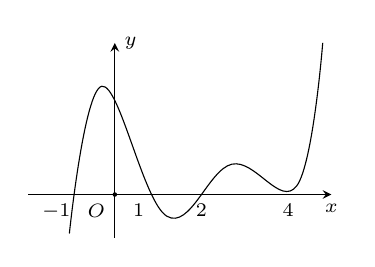
\begin{tikzpicture}[>=stealth,font=\scriptsize]
            \begin{scope}[scale=0.55]
                \draw[->] (0,-1)--(0,3.5)node[right]{\scriptsize $y$};
                \draw[->] (-2,0)--(5,0)node[below]{\scriptsize $x$};
                \fill (0,0) node[below left]{\scriptsize  $O$} circle(1.5pt);
                \draw (-0.8,0) node[below left]{ $-1$} (0.9,0) node[below left]{ $1$} (2,0) node[below]{ $2$} (4,0) node[below]{ $4$};
                \clip (-2,-1) rectangle (5,3.5);
                \draw[] plot[smooth,tension=.65] coordinates{(-1.05,-0.9) (-0.3,2.5) (1.2,-0.5) (2.7,0.7) (4.2,0.2) (4.8,3.5)};
            \end{scope}
        \end{tikzpicture}
    }
    \loigiai{
        Đặt $g(x)=f(1-2x)$\\
        Dựa vào đồ thị, ta thấy $f'(x)=0$ có nghiệm $x_1=-1,x_2=1,x_3=2$ và $x_4=4$ nên $f'(x)$ có dạng $$f'(x)=k(x+1)(x-1)(x-2)(x-4)$$
        Khi đó $g'(x)=-2f'(1-2x)=-2k(2-2x)(-2x)(-1-2x)(-3-2x)^2$
        $$g'(x)=0 \Leftrightarrow \hoac{&x=1\\&x=0\\&x=-\dfrac{1}{2}\\&x=-\dfrac{3}{2} \text{ (kép)}}$$
        Bảng xét dấu $g'(x)$
        \begin{center}
            \begin{tikzpicture}[every node/.style={circle,fill=white,inner sep=0pt},arrow/.style={>=stealth,->,shorten <= 0.3cm,shorten >= 0.3cm},font=\footnotesize,xscale=1,yscale=1]
                \def\mnumline{1} %Số dòng
                \def\mnumcol{11} %Số cột
                \foreach \j in {0,...,\mnumline}
                \foreach \i in {0,...,\mnumcol}{
                    \coordinate (\j\i) at (\i,-\j);
                }
                \pgfmathsetmacro\yline{\mnumline/2-1}
                \path node at (00){$x$} node at (10){$g'(x)$};
                \foreach \x/\mnamex in {01/$-\infty$,03/$-\dfrac{3}{2}$,05/$-\dfrac{1}{2}$,07/$0$,09/$1$,0\mnumcol/$+\infty$} \path node at (\x) {\mnamex};
                \foreach \dy/\mnamedy in {12/$-$,13/$0$,14/$-$,15/$0$,16/$+$,17/$0$,18/$-$,19/$0$,110/$+$} \path node at (\dy) {\mnamedy};
                \draw[thick] (-.5,.5)rectangle([xshift=0.5cm,yshift=-0.5cm]\mnumline\mnumcol) ([xshift=-0.5cm,yshift=-0.5cm]00)--([xshift=0.5cm,yshift=-0.5cm]0\mnumcol)  ([xshift=0.5cm,yshift=0.5cm]00)--([xshift=0.5cm,yshift=-0.5cm]\mnumline0);
            \end{tikzpicture}
        \end{center}
        Dựa vào bảng xét dấu, ta thấy $g'(x)$ đổi dấu 3 lần nên $y=f(1-2x)$ có 3 cực trị.
    }
\end{ex}
\begin{ex}%[2D1K2-2]
    \immini{Cho hàm số $ f(x) $ có đạo hàm là $ f'(x) $. Đồ thị của hàm số $ y=f'(x) $ như hình vẽ bên. Khi đó hàm số $ y=f(x^2) $ có bao nhiêu điểm cực trị?
        \choice[2]
        {$2$}
        {$4$}
        {\True $3$}
        {$5$}}
    {
        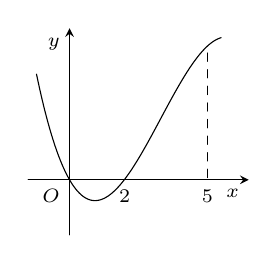
\begin{tikzpicture}[line join=round, line cap=round,>=stealth,font=\scriptsize]
            \begin{scope}[scale=0.35]
                \tikzset{label style/.style={font=\footnotesize}}
                \def \xmin{-1.5}
                \def \xmax{6.5}
                \def \ymin{-2}
                \def \ymax{5.5}
                \def \hamso{-0.11*(\x)^3+1.09*(\x)^2-1.73*(\x)}
                \draw[->] (\xmin,0)--(\xmax,0) node[below left] {$x$};
                \draw[->] (0,\ymin)--(0,\ymax) node[below left] {$y$};
                \draw (0,0) node [below left] {$O$};
                \begin{scope}
                    \clip (\xmin+0.01,\ymin+0.01) rectangle (\xmax-0.01,\ymax-0.01);
                    \draw[samples=350,domain=-1.2:5.5,smooth,variable=\x] plot (\x,{\hamso});
                \end{scope}
                \draw [dashed] (5,4.6)--(5,0) node[below]{$5$} (2,0) node[below]{$2$};
            \end{scope}
        \end{tikzpicture}
    }
    \loigiai{$ y'=2xf'(x^2) $. Cho $ y'=0 \Leftrightarrow \hoac{&x=0\\&f'(x^2)=0} \Leftrightarrow \hoac{&x=0\\&x^2=0\\&x^2=2} \Leftrightarrow \hoac{&x=0\\&x=0 \text{ (nghiệm kép)}\\&x=\pm \sqrt{2}} $.\\
        $ y'=0 $ có 3 nghiệm bội bậc lẻ nên hàm số có 3 điểm cực trị.
    }
\end{ex}
\begin{ex}%[2D1K2-6]
    \immini{	Cho hàm số $y=f(x)$ xác định trên $\mathbb{R}$ và hàm số $y=f'(x)$ có đồ thị như hình vẽ. Hàm số $y=f(1-x^2)$ đạt cực đại tại điểm nào sau đây?
        \choice[2]
        {$x=-1$}
        {\True $x=\pm \sqrt{2}$}
        {$x=3$}
        {$x=0$}}{
        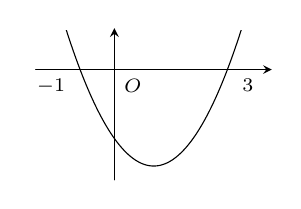
\begin{tikzpicture}[>=stealth, font=\scriptsize, line join=round, line cap=round,y=0.7cm]
            \begin{scope}[scale=.5]
                \def\a{1} \def\b{-2} \def\c{-2.5} % Hệ số
                \def\xmin{-2} \def\xmax{4}
                \def\ymin{-4} \def\ymax{1.5}
                %\draw[color=gray!50,dashed] (\xmin,\ymin) grid (\xmax,\ymax);
                \draw[->] (\xmin,0)--(\xmax,0);
                \draw[->] (0,\ymin)--(0,\ymax);
                \node at (0,0) [below right]{$O$};
                \node at (-1,0) [below left]{$-1$};
                \node at (3,0) [below right]{$3$};
                \clip (\xmin+0.1,\ymin+0.1) rectangle (\xmax-0.5,\ymax-0.1);
                \draw[smooth,samples=300,domain=-1.3:3.3] plot(\x,{\a*(\x)^2+\b*(\x)+\c});
            \end{scope}
    \end{tikzpicture}}
    \loigiai{Đặt $g(x)=f(1-x^2)$\\
        Khi đó $g'(x)=-2x\cdot f'(1-x^2)$\\
        Cho $g'(x)=0 \Leftrightarrow -2x \cdot f'(1-x^2) =0$
        $$ \Leftrightarrow \hoac{&x=0\\&f'(1-x^2)=0 \Leftrightarrow \hoac{&1-x^2=-1\Leftrightarrow x^2=2 \Leftrightarrow x=\pm \sqrt{2}\\&1-x^2=3}}$$
        Bảng xét dấu
        \begin{center}
            \begin{tikzpicture}[every node/.style={circle,fill=white,inner sep=0pt},arrow/.style={>=stealth,->,shorten <= 0.3cm,shorten >= 0.3cm},font=\footnotesize,xscale=1.4,yscale=.8]
                \def\mnumline{3} %Số dòng
                \def\mnumcol{9} %Số cột
                \foreach \j in {0,...,\mnumline}
                \foreach \i in {0,...,\mnumcol}{
                    \coordinate (\j\i) at (\i,-\j);
                    %	\draw[gray!30] ([xshift=-0.5cm,yshift=0.5cm]\j\i)--([xshift=0.5cm,yshift=0.5cm]\j\i)--([xshift=0.5cm,yshift=-0.5cm]\j\i)--([xshift=-0.5cm,yshift=-0.5cm]\j\i)--cycle (\j\i)node[]{\j\i}; %Ẩn lệnh này sau khi hoàn thành BBT
                }
                \pgfmathsetmacro\yline{\mnumline/2-1}
                \path node at (00){$x$} node at (10){$-x$} node at (20){\scriptsize $f'(1-x^2)$} node at (30){$g'(x)$};
                \foreach \x/\mnamex in {01/$-\infty$,03/$-\sqrt{2}$,05/$0$,07/$\sqrt{2}$,0\mnumcol/$+\infty$} \path node at (\x) {\mnamex};
                \foreach \dy/\mnamedy in {12/$-$,13/$0$,14/$+$,16/$+$} \path node at (\dy) {\mnamedy};
                \path node at ($(12)$){$+$} node at ($(13)$){$|$} node at ($(14)$){$+$} node at ($(15)$){$0$} node at ($(16)$){$-$} node at ($(17)$){$|$} node at ($(18)$){$-$} node at ($(22)$){$+$} node at ($(23)$){$0$} node at ($(24)$){$-$} node at ($(25)$){$|$} node at ($(26)$){$-$} node at ($(27)$){$0$} node at ($(28)$){$+$} node at ($(32)$){$+$} node at ($(33)$){$0$} node at ($(34)$){$-$} node at ($(35)$){$0$} node at ($(36)$){$+$} node at ($(37)$){$0$} node at ($(38)$){$-$};
                \draw[thick] (-.5,.5)rectangle([xshift=0.5cm,yshift=-0.5cm]\mnumline\mnumcol) ([xshift=-0.5cm,yshift=-0.5cm]00)--([xshift=0.5cm,yshift=-0.5cm]0\mnumcol) ([xshift=-0.5cm,yshift=-0.5cm]10)--([xshift=0.5cm,yshift=-0.5cm]1\mnumcol)

                ([xshift=-0.5cm,yshift=-0.5cm]20)--([xshift=0.5cm,yshift=-0.5cm]2\mnumcol)

                ([xshift=0.5cm,yshift=0.5cm]00)--([xshift=0.5cm,yshift=-0.5cm]\mnumline0); %Lệnh tự động kẻ bảng
            \end{tikzpicture}
        \end{center}
        Dựa vào bảng xét dấu ta xác định được hàm số đạt cực đại tại $x=\pm \sqrt{2}$.}
\end{ex}
\begin{ex}%[2D1K2-6]
    \immini{Cho hàm số $y=f(x)$ có đồ thị hàm $f'(x)=ax^2+bx+c$ như hình bên dưới. Hỏi hàm số $y=f(x-x^2)$ có bao nhiêu cực trị?
        \choice[2]
        {$0$}
        {\True $1$}
        {$2$}
        {$3$}}{
        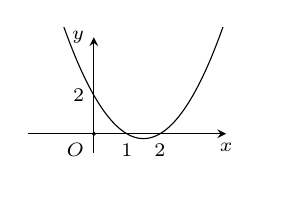
\begin{tikzpicture}[>=stealth,x=1.2cm,y=0.7cm,font=\scriptsize]
            \begin{scope}[scale=0.35]
                \clip (-2,-2) rectangle (5,5.5);
                \def\a{1}
                \def\b{-3}
                \def\c{2}
                \draw[->] (-2,0) -- (4,0) node[below] { $x$};
                \draw[->] (0,-1) -- (0,5) node[left] {$y$};
                \draw (0,0)node[below left]{ $O$} circle(1.5pt);
                \draw (1,0) node[below]{$1$} (2,0) node[below]{  $2$} (0,2) node[left]{$2$};
                \pgfmathsetmacro\xdinh{-(\b)/2*(\a)}
                \pgfmathsetmacro\ydinh{(4*(\a)*(\c)-(\b)^2)/(4*(\a))}
                \draw[samples=150,smooth,domain=-5:5] plot(\x,{\a*(\x)^2+(\b)*\x+(\c)});
            \end{scope}
        \end{tikzpicture}
    }
    \loigiai{
        Đặt $g(x)=f\left(x-x^2\right)$\\
        Dựa vào đồ thị ta thấy $f'(x)=0$ có hai nghiệm $x_1=1,x_2=2$ nên $f'(x)$ có dạng $$f'(x)=k(x-1)(x-2)$$
        Khi đó $g'(x)=(1-2x)f'\left(x-x^2\right)=0$
        $$ \Leftrightarrow \hoac{&1-2x=0\\&f'\left(x-x^2\right)=0} \Leftrightarrow \hoac{&x=\dfrac{1}{2}\\&x-x^2=1\\&x-x^2=2} \Leftrightarrow \hoac{&x=\dfrac{1}{2}\\& \text{ vô nghiệm}\\&\text{ vô nghiệm.}}$$
        Bảng xét dấu
        \begin{center}
            \begin{tikzpicture}[every node/.style={circle,fill=white,inner sep=0pt},arrow/.style={>=stealth,->,shorten <= 0.3cm,shorten >= 0.3cm},font=\footnotesize,xscale=1,yscale=1]
                \def\mnumline{1} %Số dòng
                \def\mnumcol{5} %Số cột
                \foreach \j in {0,...,\mnumline}
                \foreach \i in {0,...,\mnumcol}{
                    \coordinate (\j\i) at (\i,-\j);
                }
                \pgfmathsetmacro\yline{\mnumline/2-1}
                \path node at (00){$x$} node at (10){$g'(x)$};
                \foreach \x/\mnamex in {01/$-\infty$,03/$\dfrac{1}{2}$,0\mnumcol/$+\infty$} \path node at (\x) {\mnamex};
                \foreach \dy/\mnamedy in {12/$+$,13/$0$,14/$-$} \path node at (\dy) {\mnamedy};
                \draw[thick] (-.5,.5)rectangle([xshift=0.5cm,yshift=-0.5cm]\mnumline\mnumcol) ([xshift=-0.5cm,yshift=-0.5cm]00)--([xshift=0.5cm,yshift=-0.5cm]0\mnumcol)  ([xshift=0.5cm,yshift=0.5cm]00)--([xshift=0.5cm,yshift=-0.5cm]\mnumline0);
            \end{tikzpicture}
        \end{center}
        Dựa vào bảng xét dấu, ta thấy $g(x)$ có 1 cực đại.
    }
\end{ex}
\begin{ex}%[2D1K2-2]
    \immini{Cho hàm số bậc bốn $y=f(x)$. Hàm số $y=f'(x)$
        có đồ thị như hình bên. Số điểm cực trị của hàm số $y=f\left(\sqrt{x^{2}+2 x+2}\right)$ là
        \choice[2]
        {$1$}
        {$2$}
        {$4$}
        {\True $3$}}
    {
        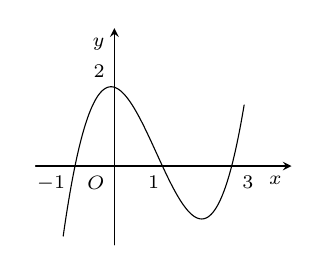
\begin{tikzpicture}[line join=round, line cap=round,>=stealth,font=\scriptsize]
            \begin{scope}[scale=0.5]
                \tikzset{label style/.style={font=\footnotesize}}
                \def \xmin{-2}
                \def \xmax{4.5}
                \def \ymin{-2}
                \def \ymax{3.5}
                \def \hamso{0.55*(\x)^3-1.76*(\x)^2-0.31*(\x)+2}
                \draw[->] (\xmin,0)--(\xmax,0) node[below left] {$x$};
                \draw[->] (0,\ymin)--(0,\ymax) node[below left] {$y$};
                \draw (0,0) node [below left] {$O$};
                \begin{scope}
                    \clip (\xmin+0.01,\ymin+0.01) rectangle (\xmax-0.01,\ymax-0.01);
                    \draw[samples=350,domain=-1.3:3.3,smooth,variable=\x] plot (\x,{\hamso});
                \end{scope}
                \draw (-1,0) node[below left]{$-1$} (1,0) node[below]{$1$} (3,0) node[below right]{$3$} (0,2) node[above left]{$2$};
            \end{scope}
        \end{tikzpicture}
    }
    \loigiai{
        $ y'=\dfrac{x+1}{\sqrt{x^2+2x+2}}f'(\sqrt{x^2+2x+2}) $.\\$ y'=0 \Leftrightarrow \hoac{&x=-1\\&f'(\sqrt{x^2+2x+2})=0} \Leftrightarrow \hoac{&x=-1\\&\sqrt{x^2+2x+2}=-1\\&\sqrt{x^2+2x+2}=1\\&\sqrt{x^2+2x+2}=3} \Leftrightarrow \hoac{&x=-1\\&x^2+2x+1=0\\&x^2+2x-7=0}\Leftrightarrow \hoac{&x=-1\\&x=-1 \text{ (nghiệm kép)}\\&x=-1\pm 2\sqrt{2}} $\\
        $ y'=0 $ có 3 nghiệm bội bậc lẻ nên hàm số có 3 điểm cực trị.
    }
\end{ex}
\begin{ex}%[2D1K2-2]
    \immini{Cho hàm số $ y=f(x) $ liên tục trên $ (a,b) $ và có đồ thị như hình bên. Số điểm cực trị của hàm số $ y=\left[f(x)\right]^2 $ trên $ (a;b) $ là
        \choice[2]
        {$4$}
        {$6$}
        {$2$}
        {\True $5$}}
    {
        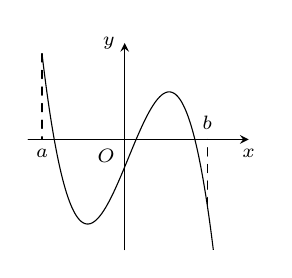
\begin{tikzpicture}[line join=round, line cap=round,>=stealth,font=\scriptsize]
            \begin{scope}[scale=.35]
                \def \xmin{-3.5}
                \def \xmax{4.5}
                \def \ymin{-4}
                \def \ymax{3.5}
                \def \hamso{-0.37*(\x)^3+0.15*(\x)^2+2.41*(\x)-1}
                \draw[->] (\xmin,0)--(\xmax,0) node[below] {$x$};
                \draw[->] (0,\ymin)--(0,\ymax) node[left] {$y$};
                \draw (0,0) node [below left] {$O$};
                \clip (\xmin+0.01,\ymin+0.01) rectangle (\xmax-0.01,\ymax-0.01);
                \draw[samples=350,domain=-3:4,smooth,variable=\x] plot (\x,{\hamso});
                \draw[dashed] (-3,3.11)--(-3,0) node[below]{$a$} (3,-2.41)--(3,0) node[above]{$b$};
            \end{scope}
        \end{tikzpicture}
    }
    \loigiai{\immini{$ y=\left(f(x)\right)^2 $ nên $ y'=2f(x)f'(x) $.\\$ y'=0 \Leftrightarrow \hoac{&f(x)=0\\&f'(x)=0} \Leftrightarrow \hoac{&x=x_1,\ x=x_2,\ x=x_3\\&x=c,\ x=d}$.\\
            $ y'=0 $ có 5 nghiệm bội bậc lẻ thuộc $ (a,b) $ nên Số điểm cực trị của hàm số $ y=\left(f(x)\right)^2 $ trên $ (a;b) $ là 5.}
        {
            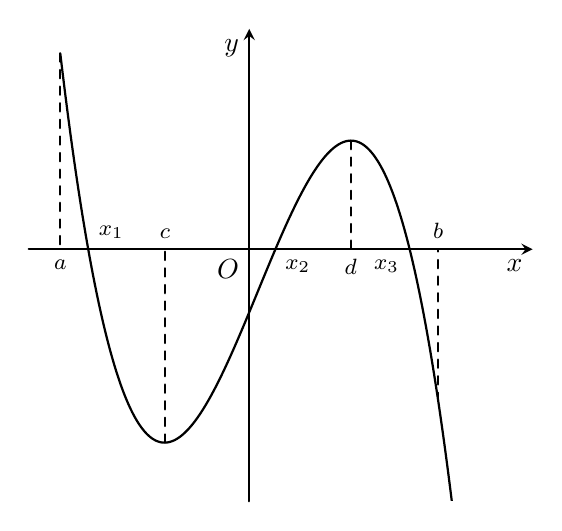
\begin{tikzpicture}[line join=round, line cap=round,>=stealth,thick,scale=0.8]
                \tikzset{label style/.style={font=\footnotesize}}
                \def \xmin{-3.5}
                \def \xmax{4.5}
                \def \ymin{-4}
                \def \ymax{3.5}
                \def \hamso{-0.37*(\x)^3+0.15*(\x)^2+2.41*(\x)-1}
                \draw[->] (\xmin,0)--(\xmax,0) node[below left] {$x$};
                \draw[->] (0,\ymin)--(0,\ymax) node[below left] {$y$};
                \draw (0,0) node [below left] {$O$};
                \begin{scope}
                    \clip (\xmin+0.01,\ymin+0.01) rectangle (\xmax-0.01,\ymax-0.01);
                    \draw[samples=350,domain=-3:4,smooth,variable=\x] plot (\x,{\hamso});
                \end{scope}
                \draw[dashed] (-3,3.11)--(-3,0) node[below]{\footnotesize $a$} (3,-2.41)--(3,0) node[above]{\footnotesize $b$} (2.54,0) node[below left]{\footnotesize $x_3$} (0.41,0) node[below right]{\footnotesize $x_2$} (-2.55,0) node[above right]{\footnotesize $x_1$} (-1.34,-3.07) -- (-1.34,0) node[above]{\footnotesize $c$} (1.61,1.72)--(1.61,0) node[below]{\footnotesize $d$};
            \end{tikzpicture}
        }
    }
\end{ex}
\begin{ex}%[2D1G2-1]
    \immini{Cho hàm số $y=f(x)$ có đạo hàm trên $\mathbb{R}$ và có bảng xét dấu $f'(x)$ như hình bên. Hàm số $y=f\left(x^{2}-2 x\right)$ có bao nhiêu điểm cực tiểu?
        \choice
        {\True $1$}
        {$2$}
        {$3$}
        {$4$}}{
\begin{tikzpicture}
            \tkzTabInit[lgt=1,espcl=1.2]
            {$x$ /.7, $y'$ /.7}
            {$-\infty$,$-2$,$1$,$3$,$+\infty$}
            \tkzTabLine{ ,-,0,+,0,+,0,-, }
    \end{tikzpicture}}
    \loigiai{$ y'=(2x-2)f'(x^2-2x) $.
        \begin{eqnarray*}
            y'=0 	&\Leftrightarrow& \hoac{&x=1\\&f'(x^2-2x)=0}\\
            &\Leftrightarrow& \hoac{&x=1\\&x^2-2x=-2 \text{ (vô nghiệm)}\\&x^2-2x=1 \text{ (nghiệm bội bậc chẵn)}\\&x^2-2x=3} \\
            &\Leftrightarrow& \hoac{&x=1\\&x=1-\sqrt{2} \text{ (nghiệm bội bậc chẵn)}\\&x=1+\sqrt{2} \text{ (nghiệm bội bậc chẵn)}\\&x=3, \ x=-1.}
        \end{eqnarray*}
        $ y'=0 $ có 3 nghiệm bội bậc lẻ, khi đó $ y' $ đổi dấu qua các nghiệm này.\\
        $ y'=0 $ có 2 nghiệm bội bậc chẵn và $ y' $ sẽ không đổi dấu qua các nghiệm này.\\
        Tại $ x=4 $ thì $ y'(4)=(2\cdot 4 -2)f'(4^2-2\cdot 4)=6f'(8)<0 $.\\
        Bảng xét dấu
        \begin{center}
            
\begin{tikzpicture}
                \tkzTabInit[lgt=1,espcl=1.2]
                {$x$ /1, $y'$ /1}
                {$-\infty$,$-1$,$1-\sqrt{2}$,$1+\sqrt{2}$,$3$,$+\infty$}
                \tkzTabLine{ ,-,0,+,0,+,0,+,0,-, }
            \end{tikzpicture}
        \end{center}
        Vậy hàm số có 1 điểm cực tiểu.
    }
\end{ex}
\begin{ex}%[2D1K2-6]
    \immini{Cho hàm số $f(x)$ có bảng biến thiên bên dưới. Trên khoảng $(-\sqrt{5};\sqrt{5})$ thì hàm số $y=f(x^2)$ đạt cực đại tại điểm nào sau đây?\choice
        {$x=\sqrt{2}$}
        {$x=-\sqrt{2}$}
        {\True $x=0$}
        {$x=2$}}{
\begin{tikzpicture}
            \tkzTabInit[nocadre=false,lgt=1,espcl=1.6,deltacl=0.5]{$x$/.7 ,$f$/.7}
            {$-\infty$ , $0$ , $2$ , $+\infty$}
            \tkzTabLine{  , + , 0, - , 0 , +  }
    \end{tikzpicture}}
    \loigiai{Đặt $g(x)=f(x^2)$.\\
        Khi đó $g'(x)=2x \cdot f'(x^2)$.\\
        Cho $g'(x)=0 \Leftrightarrow 2x \cdot f'(x^2) =0 \Leftrightarrow
        \hoac{&x=0\\&f'(x^2)=0 \Leftrightarrow \hoac{x^2=0\\x^2=2} \Leftrightarrow \hoac{x=0\\x=\pm \sqrt{2}}}$\\
        Bảng xét dấu
        \begin{center}
            \begin{tikzpicture}[every node/.style={circle,fill=white,inner sep=0pt},arrow/.style={>=stealth,->,shorten <= 0.3cm,shorten >= 0.3cm},font=\footnotesize,xscale=1,yscale=.7]
                \def\mnumline{3} %Số dòng
                \def\mnumcol{9} %Số cột
                \foreach \j in {0,...,\mnumline}
                \foreach \i in {0,...,\mnumcol}{
                    \coordinate (\j\i) at (\i,-\j);
                }
                \pgfmathsetmacro\yline{\mnumline/2-1}
                \path node at (00){$x$} node at (10){$x$} node at (20){$f'(x^2)$} node at (30){$g'(x)$};
                \foreach \x/\mnamex in {01/$-\sqrt{5}$,03/$-\sqrt{2}$,05/$0$,07/$\sqrt{2}$,0\mnumcol/$\sqrt{5}$} \path node at (\x) {\mnamex};
                \foreach \dy/\mnamedy in {12/$-$,13/$0$,14/$+$,16/$+$} \path node at (\dy) {\mnamedy};
                \path node at ($(12)$){$-$} node at ($(13)$){$|$} node at ($(14)$){$-$} node at ($(15)$){$0$} node at ($(16)$){$+$} node at ($(17)$){$|$} node at ($(18)$){$+$} node at ($(22)$){$+$} node at ($(23)$){$0$} node at ($(24)$){$-$} node at ($(25)$){$0$} node at ($(26)$){$-$} node at ($(27)$){$0$} node at ($(28)$){$+$} node at ($(32)$){$-$} node at ($(33)$){$0$} node at ($(34)$){$+$} node at ($(35)$){$0$} node at ($(36)$){$-$} node at ($(37)$){$0$} node at ($(38)$){$+$};
                \draw[thick] (-.5,.5)rectangle([xshift=0.5cm,yshift=-0.5cm]\mnumline\mnumcol) ([xshift=-0.5cm,yshift=-0.5cm]00)--([xshift=0.5cm,yshift=-0.5cm]0\mnumcol) ([xshift=-0.5cm,yshift=-0.5cm]10)--([xshift=0.5cm,yshift=-0.5cm]1\mnumcol)

                ([xshift=-0.5cm,yshift=-0.5cm]20)--([xshift=0.5cm,yshift=-0.5cm]2\mnumcol)

                ([xshift=0.5cm,yshift=0.5cm]00)--([xshift=0.5cm,yshift=-0.5cm]\mnumline0); %Lệnh tự động kẻ bảng
            \end{tikzpicture}
        \end{center}
        Dựa vào bảng xét dấu ta xác định được hàm số đạt cực đại tại $x=0$.
    }
\end{ex}
\begin{ex}%[2D1K2-6]
    \immini{Cho hàm số $f(x)$ có bảng biến thiên bên dưới. Hàm số $y=f(x^2-2)$ đạt cực đại tại điểm nào sau đây?
        \choice
        {$x=-2$}
        {$x=-1$}
        {\True $x=0$}
        {$x=2$}}{
\begin{tikzpicture}
            \tkzTabInit[nocadre=false,lgt=1,espcl=1.6,deltacl=0.5]{$x$/.7 ,$f$/.7}
            {$-\infty$ , $-1$ , $2$ , $+\infty$}
            \tkzTabLine{  , - , 0, - , 0 , +  }
    \end{tikzpicture}}
    \loigiai{Đặt $g(x)=f(x^2-2)$\\
        Khi đó $g'(x)=2x \cdot f'(x^2-2)$\\
        Cho $g'(x)=0 \Leftrightarrow 2x \cdot f'(x^2-2) =0$
        $$ \Leftrightarrow \hoac{&x=0\\&f'(x^2-2)=0 \Leftrightarrow \hoac{&x^2-2=-1\\&x^2-2=2} \Leftrightarrow \hoac{x^2=1\\x^2=4} \Leftrightarrow \hoac{x=\pm 1\\x=\pm 2}}$$
        Bảng xét dấu
        \begin{center}
            \begin{tikzpicture}[every node/.style={circle,fill=white,inner sep=0pt},arrow/.style={>=stealth,->,shorten <= 0.3cm,shorten >= 0.3cm},font=\footnotesize,xscale=1,yscale=1]
                \def\mnumline{3} %Số dòng
                \def\mnumcol{14} %Số cột
                \foreach \j in {0,...,\mnumline}
                \foreach \i in {0,...,\mnumcol}{
                    \coordinate (\j\i) at (\i,-\j);
                }
                \pgfmathsetmacro\yline{\mnumline/2-1}
                \path node at ([xshift=0.5cm]00){$x$} node at ([xshift=0.5cm]10){$x$}  node at ([xshift=0.5cm]20){$f'\left(x^2-2\right)$} node at ([xshift=0.5cm]\mnumline0){$g'(x)$};
                \foreach \x/\mnamex in {02/$-\infty$,04/$-2$,06/$-1$,08/$0$,010/$1$,012/$2$,0\mnumcol/$+\infty$} \path node at (\x) {\mnamex};
                \foreach \dy/\mnamedy in {13/$-$,14/$0$,15/$+$,16/$+$} \path node at (\dy) {\mnamedy};
                \path node at ($(13)$){$-$} node at ($(14)$){$|$} node at ($(15)$){$-$} node at ($(16)$){$|$} node at ($(17)$){$-$} node at ($(18)$){$0$} node at ($(19)$){$+$} node at ($(110)$){$|$} node at ($(111)$){$+$} node at ($(112)$){$|$} node at ($(113)$){$+$}
                node at ($(23)$){$+$} node at ($(24)$){$0$} node at ($(25)$){$-$} node at ($(26)$){$0$} node at ($(27)$){$-$} node at ($(28)$){$|$} node at ($(29)$){$-$} node at ($(210)$){$0$} node at ($(211)$){$-$} node at ($(212)$){$0$} node at ($(213)$){$+$}
                node at ($(33)$){$-$} node at ($(34)$){$0$} node at ($(35)$){$+$} node at ($(36)$){$0$} node at ($(37)$){$+$} node at ($(38)$){$0$} node at ($(39)$){$-$} node at ($(310)$){$0$} node at ($(311)$){$-$} node at ($(312)$){$0$} node at ($(313)$){$+$};
                \draw[thick] (-.5,.5)rectangle([xshift=0.5cm,yshift=-0.5cm]\mnumline\mnumcol) ([xshift=-0.5cm,yshift=-0.5cm]00)--([xshift=0.5cm,yshift=-0.5cm]0\mnumcol)
                ([xshift=-0.5cm,yshift=-0.5cm]20)--([xshift=0.5cm,yshift=-0.5cm]2\mnumcol)
                ([xshift=-0.5cm,yshift=-0.5cm]10)--([xshift=0.5cm,yshift=-0.5cm]1\mnumcol) ([xshift=0.5cm,yshift=0.5cm]01)--([xshift=0.5cm,yshift=-0.5cm]\mnumline1); %Lệnh tự động kẻ bảng
            \end{tikzpicture}
        \end{center}
        Dựa vào bảng xét dấu ta xác định được hàm số đạt cực đại tại $x=0$.
    }
\end{ex}
\begin{ex}%[2D1K2-1]
    Cho hàm số $ y=f(x) $ có đạo hàm $ f'(x)=x^2(x-1)(x-4)^2 $. Khi đó hàm số $ y=f(x^2) $ có bao nhiêu điểm cực trị?
    \choice
    {$4$}
    {\True $3$}
    {$5$}
    {$2$}
    \loigiai{$ f'(x)=0 \Leftrightarrow x=1 $ (nghiệm đơn), $ x=0 $ (nghiệm kép), $ x=4 $ (nghiệm kép).\\
        $ y=f(x^2) $ thì $ y'=2xf'(x^2) $.\\$y'=0 \Leftrightarrow \hoac{&x=0\\&x^2=1\\&x^2=0 \text{ (nghiệm kép)}\\&x^2=4 \text{ (nghiệm kép)}} \Leftrightarrow \hoac{&x=0\\&x=\pm 1\\&x=0 \text{ (nghiệm bội chẵn)}\\&x=\pm 2 \text{ (nghiệm bội chẵn).}} $\\
        Vậy hàm số có 3 điểm cực trị.
    }
\end{ex}
\begin{ex}%[2D1K2-6]
    Cho hàm $f(x)$ có đạo hàm $f'(x)=x^2-2x,\forall x\in \mathbb{R}$. Hàm số $y=f\left(1-\dfrac{1}{2}x\right)+4x$ có bao nhiêu điểm cực trị?
    \choice
    {0}
    {1}
    {\True 2}
    {3}
    \loigiai{Ta có $y'=-\dfrac{1}{2}f'\left(1-\dfrac{1}{2}x\right)+4$\\
        $y'=0 \Leftrightarrow
        f'\left(1-\dfrac{1}{2}x\right)=8\Leftrightarrow \left(1-\dfrac{1}{2}x\right)^2-2\left(1-\dfrac{1}{2}x\right)=8 \Leftrightarrow \dfrac{1}{4}x^2-9=0
        \Leftrightarrow \hoac{&x=-6\\&x=6}$\\
        Bảng xét dấu
        \begin{center}
            \begin{tikzpicture}[every node/.style={circle,fill=white,inner sep=0pt},arrow/.style={>=stealth,->,shorten <= 0.3cm,shorten >= 0.3cm},font=\footnotesize,xscale=1,yscale=1]
                \def\mnumline{1} %Số dòng
                \def\mnumcol{7} %Số cột
                \foreach \j in {0,...,\mnumline}
                \foreach \i in {0,...,\mnumcol}{
                }
                \pgfmathsetmacro\yline{\mnumline/2-1}
                \path node at (00){$x$} node at (10){$y'$};
                \foreach \x/\mnamex in {01/$-\infty$,03/$-6$,05/$6$,0\mnumcol/$+\infty$} \path node at (\x) {\mnamex};
                \foreach \dy/\mnamedy in {12/$+$,13/$0$,14/$-$,15/$0$,16/$+$} \path node at (\dy) {\mnamedy};
                \draw[thick] (-.5,.5)rectangle([xshift=0.5cm,yshift=-0.5cm]\mnumline\mnumcol) ([xshift=-0.5cm,yshift=-0.5cm]00)--([xshift=0.5cm,yshift=-0.5cm]0\mnumcol)  ([xshift=0.5cm,yshift=0.5cm]00)--([xshift=0.5cm,yshift=-0.5cm]\mnumline0); %Lệnh tự động kẻ bảng
            \end{tikzpicture}
        \end{center}
        Vậy hàm số $y=f\left(1-\dfrac{1}{2}x\right)+4x$ có 2 điểm cực trị.}
\end{ex}
\begin{ex}%[2D1G2-1]
    Cho hàm số $ y=f(x) $ có đạo hàm $ f'(x)=(x-1)^2(x^2-2x) $, với mọi $ x \in \mathbb{R} $. Có bao nhiêu giá trị nguyên dương của tham số $m$ để hàm số $ y=f(x^2-8x+m) $ có 5 điểm cực trị?
    \choice
    {\True $15$}
    {$16$}
    {$17$}
    {$18$}
    \loigiai{$ f'(x)=0 \Leftrightarrow x=1 $ (nghiệm kép), $ x=0 $ (nghiệm đơn), $ x=2 $ (nghiệm đơn).\\
        $ y=f(x^2-8x+m) $ thì $ y'=(2x-8)f'(x^2-8x+m) $.\\$y'=0 \Leftrightarrow \hoac{&x=4\\&x^2-8x+m=1 \text{ (nghiệm kép)}\\&x^2-8x+m=0 \quad (1)\\&x^2-8x+m=2 \quad (2)} $.\\
        Hàm số có 5 điểm cực trị $ \Leftrightarrow (1) $ có 2 nghiệm phân biệt khác 4 và $ (2) $ có 2 nghiệm phân biệt khác 4.\\$(1) $ có 2 nghiệm phân biệt khác 4 $ \Leftrightarrow \heva{&16-32+m \ne 0\\&\Delta'=16-m>0} \Leftrightarrow \heva{&m \ne 16\\&m<16}\Leftrightarrow m<16$.\\
        $(2) $ có 2 nghiệm phân biệt khác 4 $ \Leftrightarrow \heva{&16-32+m \ne 2\\&\Delta'=16-m+2>0} \Leftrightarrow \heva{&m \ne 18\\&m<18} \Leftrightarrow m<18$.\\
        Vậy ta có $ m<16 $ mà $ m $ nguyên dương nên $ m \in \{1,2,\cdots,15\} $ (15 số $ m $ thỏa mãn).
    }
\end{ex}
\begin{ex}%[2D1Y2-2]
    \immini
    {
        Cho hàm số $y=f(x)$ có đạo hàm liên tục trên $\mathbb{R}$. Đồ thị hàm số $y=f'(x)$ như hình vẽ bên. Số điểm cực trị của hàm số $y=f(x)-5x$ là
        \choice
        {$2$}
        {$3$}
        {$4$}
        {\True $1$}
    }
    {
        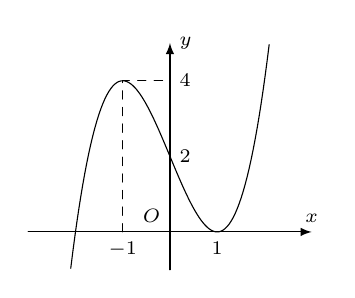
\begin{tikzpicture}[font=\scriptsize, line join=round, line cap=round, >=stealth,y=.8cm]
            \begin{scope}[scale=.6]
                \draw[->,>=latex](-3,0)--(3,0)node[above]{$x$};
                \draw[->,>=latex](0,-1)--(0,5)node[right]{$y$};
                \node[above left] at (0,0){$O$};
                \draw plot [samples=100,domain=-2.1:2.1] (\x,{(\x)^3-3*(\x)+2});
                \foreach\i in{-1,1}{\node[below] at (\i,0){$\i$};}
                \foreach\i in{4,2}{\node[right] at (0,\i){$\i$};}
                \draw[dashed](-1,0)--(-1,4)--(0,4);
            \end{scope}
        \end{tikzpicture}
    }
    \loigiai
    {
        Gọi $g(x)=f(x)-5x$. Ta có đạo hàm $g'(x)=f'(x)-5$. Bảng biến thiên của $g'(x)$ như hình dưới.
        \begin{center}
            
\begin{tikzpicture}
                \tkzTabInit[nocadre=false,lgt=1.2,espcl=2.5,deltacl=0.6]
                {$x$/1, $f'(x)$/2, $g'(x)$/2}
                {$-\infty$, $-1$, $1$, $+\infty$}
                \tkzTabVar{-/ $-\infty$, +/$4$, -/$0$, +/$+\infty$}
                \tkzTabVar{-/ $-\infty$, +/$-1$, -/$-5$, +/$+\infty$}
            \end{tikzpicture}
        \end{center}
        Ta thấy $g'(x)$ chỉ đổi dấu một lần từ âm sang dương.\\
        Vì vậy hàm số $y=f(x)-5x$ có một điểm cực trị.
    }
\end{ex}
\begin{ex}%[2D1Y2-2]
    \immini
    {
        Cho hàm số $y=f(x)$ có đạo hàm trên $\mathbb{R}$. Biết hàm số $y=f'(x)$ có đồ thị như hình vẽ. Khẳng định nào sau đây đúng về cực trị của hàm số $g(x)=f(x)+x$?
        \choice
        {Hàm số có một điểm cực đại và một điểm cực tiểu}
        {Hàm số không có điểm cực đại và một điểm cực tiểu}
        {Hàm số có một điểm cực đại và hai điểm cực tiểu}
        {\True Hàm số có hai điểm cực đại và một điểm cực tiểu}
    }
    {
        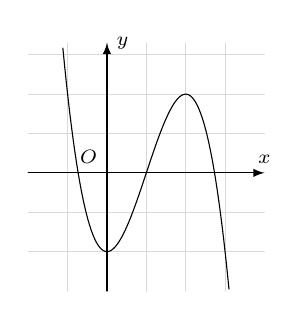
\begin{tikzpicture}[ font=\scriptsize, line join=round, line cap=round, >=stealth]
            \begin{scope}[scale=.5]
                \foreach\x in{-1,0,...,3}{\draw[color=gray!30](\x,-3)--(\x,3.3);}
                \foreach\y in{-2,-1,...,3}{\draw[color=gray!30](-2,\y)--(4,\y);}
                \draw[->,>=latex](-2,0)--(4,0)node[above]{$x$};
                \draw[->,>=latex](0,-3)--(0,3.3)node[right]{$y$};
                \node[above left] at (0,0){$O$};
                \draw plot [samples=100,domain=-1.12:3.1] (\x,{-(\x)^3+3*(\x)^2-2});
            \end{scope}
        \end{tikzpicture}
    }
    \loigiai
    {
        Ta có $g'(x)=f'(x)+1$. Bảng biến thiên của $g'(x)$ như hình dưới.
        \begin{center}
            
\begin{tikzpicture}
                \tkzTabInit[nocadre=false,lgt=1.2,espcl=2.5,deltacl=0.6]
                {$x$/1, $f'(x)$/2, $g'(x)$/2}
                {$-\infty$, $0$, $2$, $+\infty$}
                \tkzTabVar{+/ $+\infty$, -/$-2$, +/$2$, -/$-\infty$}
                \tkzTabVar{+/ $+\infty$, -/$-1$, +/$3$, -/$-\infty$}
            \end{tikzpicture}
        \end{center}
        Dựa vào bảng biến thiên của $g'(x)$, ta thấy đạo hàm đổi dấu từ dương sang âm hai lần, từ âm sang dương một lần.\\
        Do đó hàm số $g(x)$ có hai điểm cực đại và một điểm cực tiểu.
    }
\end{ex}
\begin{ex}%[2D1K2-6]
    \immini{	Cho hàm số $y=f(x)$ có đạo hàm trên $\mathbb{R}$ và có đồ thị hàm số $f'(x)$ như hình vẽ. Hàm số $y=2f(x)+x^2$ đạt cực đại tại điểm nào sau đây ?
        \choice[2]
        {\True $x=-1$}
        {$x=0$}
        {$x=1$}
        {$x=2$}}{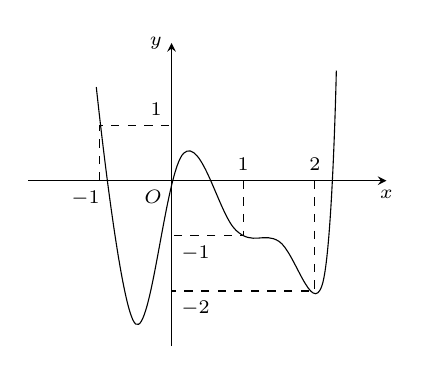
\begin{tikzpicture}[>=stealth,font=\scriptsize,x=1.3cm]
            \begin{scope}[scale=.7]
                \draw[->] (-2,0) -- (3,0) node[below] {\scriptsize $x$};
                \draw[->] (0,-3) -- (0,2.5) node[left] { $y$};
                \draw (0,0)node[below left]{$O$} (-1.2,0) node[below]{ $-1$} (0,-2) node[below right]{ $-2$} (0,1) node[above left]{$1$} (0,-1) node[below right]{  $-1$} (1,0) node[above]{$1$} (2,0) node[above]{ $2$};
                \draw plot[smooth,tension=.65] coordinates{(-1.05,1.7) (-0.5,-2.6) (0.17,0.5) (0.9,-0.9) (1.5,-1.1) (2.1,-1.9) (2.3,2)};
                \draw[dashed] (-1,0) -- (-1,1) -- (0,1) (1,0)--(1,-1)--(0,-1) (2,0)--(2,-2)--(0,-2);
            \end{scope}
    \end{tikzpicture}}
    \loigiai{
        Đặt $g(x)=2f(x)+x^2$\\
        Khi đó $g'(x)=2f'(x)+2x=0 \Leftrightarrow 2\left(f'(x)+x\right)=0 \Leftrightarrow f'(x)=-x \quad (*)$\\
        Số nghiệm của phương trình $(*)$ là số giao điểm của đồ thị hàm số $y=f'(x)$ và $y=-x$\\
        Dựa vào hình bên ta thấy có $4$ giao điểm lần lượt có tọa độ là $(-1;1),(0;0),(1;-1)$ và $(2;-2)$ \\ $ \Rightarrow (*)  \Leftrightarrow \hoac{&x=-1 \quad \text{(đơn)}\\&x=0 \quad \text{(đơn)}\\&x=1 \quad \text{(kép)}\\&x=2 \quad \text{(kép)}.}$\\
        Bảng xét dấu
        \begin{center}
            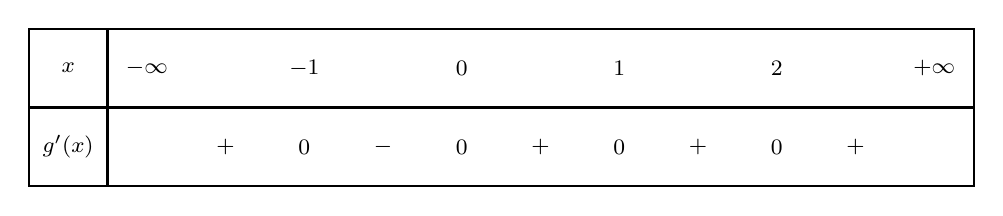
\begin{tikzpicture}[every node/.style={circle,fill=white,inner sep=0pt},arrow/.style={>=stealth,->,shorten <= 0.3cm,shorten >= 0.3cm},font=\footnotesize,xscale=1,yscale=1]
                \def\mnumline{1} %Số dòng
                \def\mnumcol{11} %Số cột
                \foreach \j in {0,...,\mnumline}
                \foreach \i in {0,...,\mnumcol}{
                    \coordinate (\j\i) at (\i,-\j);
                }
                \pgfmathsetmacro\yline{\mnumline/2-1}
                \path node at (00){$x$} node at (10){$g'(x)$};
                \foreach \x/\mnamex in {01/$-\infty$,03/$-1$,05/$0$,07/$1$,09/$2$,0\mnumcol/$+\infty$} \path node at (\x) {\mnamex};
                \foreach \dy/\mnamedy in {12/$+$,13/$0$,14/$-$,15/$0$,16/$+$,17/$0$,18/$+$,19/$0$,110/$+$} \path node at (\dy) {\mnamedy};
                \draw[thick] (-.5,.5)rectangle([xshift=0.5cm,yshift=-0.5cm]\mnumline\mnumcol) ([xshift=-0.5cm,yshift=-0.5cm]00)--([xshift=0.5cm,yshift=-0.5cm]0\mnumcol)  ([xshift=0.5cm,yshift=0.5cm]00)--([xshift=0.5cm,yshift=-0.5cm]\mnumline0);
            \end{tikzpicture}
        \end{center}
        Dựa vào bảng xét dấu, ta thấy $g(x)$ đạt cực đại tại $x=-1$.
    }
\end{ex}
\begin{ex}%[2D1K2-6]
    \immini{Hàm số $y=f(x)$ liên tục trên $\mathbb{R}$ và có đồ thị hàm số $f'(x)$ như hình vẽ bên dưới. Hàm số $y=f(x)-\dfrac{1}{3}x^3+x^2-x+2$ đạt cực đại tại điểm nào sau đây ?
        \choice[2]
        {\True $x=1$}
        {$x=-1$}
        {$x=0$}
        {$x=2$}}{\begin{tikzpicture}[>=stealth,font=\scriptsize,y=.7cm]
            \begin{scope}[scale=.8]
                \draw[->] (-2,0) -- (3,0) node[below] {\scriptsize $x$};
                \draw[->] (0,-3) -- (0,2.5) node[left] {\scriptsize $y$};
                \draw (0,0)node[below left]{ $O$}  (-1.2,0) node[below left]{ $-1$} (0,-2) node[right]{ $-2$} (0,1) node[above left]{  $1$} (1,0) node[below]{ $1$} (2,0) node[below]{ $2$};
                \draw plot [samples=100,domain=-1.1:2.2] (\x,{(\x)^3-2*(\x)^2+1});
                \draw[dashed] (-1,0) -- (-1,-2) -- (0,-2) (0,1)--(2,1)--(2,0);
            \end{scope}
    \end{tikzpicture}}
    \loigiai{
        Đặt $g(x)=f(x)-\dfrac{1}{3}x^3+x^2-x+2$	\\
        Khi đó $g'(x)=f'(x)-x^2+2x-1$.\\
        $g'(x)=0 \Leftrightarrow f'(x)=x^2-2x+1 \quad (*)$
        \immini{Số nghiệm của $(*)$ cũng chính là số giao điểm của đồ thị hàm số $y=f'(x)$ với $y=x^2-2x+1$\\
            Dựa vào hình vẽ bên, ta thấy có $3$ giao điểm lần lượt có tọa độ là $(1;0),(2;1),(0;1)$. Khi đó,
            $(*) \Leftrightarrow \hoac{&x=1\\&x=0\\&x=2.}$
        }
        {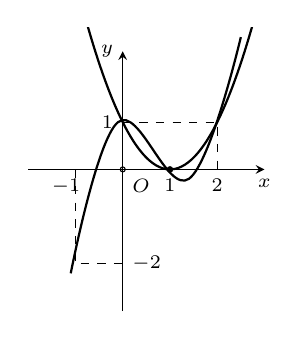
\begin{tikzpicture}[>=stealth,x=1.0cm,y=1.0cm,scale=0.6]
                \draw[->] (-2,0) -- (3,0) node[below] {\scriptsize $x$};
                \draw[->] (0,-3) -- (0,2.5) node[left] {\scriptsize $y$};
                \draw (0,0)node[below right]{\scriptsize $O$} circle(1.5pt) (-1.2,0) node[below]{\scriptsize $-1$} (0,-2) node[right]{\scriptsize  $-2$} (0,1) node[left]{\scriptsize  $1$} (1,0) node[below]{\scriptsize  $1$} (2,0) node[below]{\scriptsize  $2$};
                \def\a{1}
                \def\b{-2}
                \def\c{1}
                \pgfmathsetmacro\xdinh{-(\b)/2*(\a)}
                \pgfmathsetmacro\ydinh{(4*(\a)*(\c)-(\b)^2)/(4*(\a))}
                \fill[dashed] (\xdinh,\ydinh)circle(2pt) edge (\xdinh,0) edge (0,\ydinh);
                \clip (-2,-3)rectangle(3,3);
                \draw[thick,samples=150,smooth,domain=-5:5] plot(\x,{\a*(\x)^2+(\b)*\x+(\c)});
                \draw[thick] plot[smooth,tension=.65] coordinates{(-1.1,-2.2) (-0.1,1) (1.4,-0.2) (2.5,2.8)};
                \draw[dashed] (-1,0) -- (-1,-2) -- (0,-2) (0,1)--(2,1)--(2,0);
        \end{tikzpicture}}
        \noindent
        Bảng xét dấu
        \begin{center}
            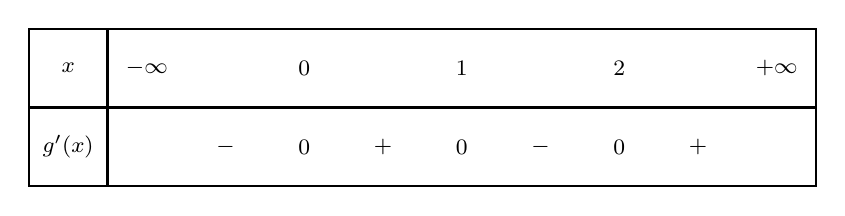
\begin{tikzpicture}[every node/.style={circle,fill=white,inner sep=0pt},arrow/.style={>=stealth,->,shorten <= 0.3cm,shorten >= 0.3cm},font=\footnotesize,xscale=1,yscale=1]
                \def\mnumline{1} %Số dòng
                \def\mnumcol{9} %Số cột
                \foreach \j in {0,...,\mnumline}
                \foreach \i in {0,...,\mnumcol}{
                    \coordinate (\j\i) at (\i,-\j);
                }
                \pgfmathsetmacro\yline{\mnumline/2-1}
                \path node at (00){$x$} node at (10){$g'(x)$};
                \foreach \x/\mnamex in {01/$-\infty$,03/$0$,05/$1$,07/$2$,0\mnumcol/$+\infty$} \path node at (\x) {\mnamex};
                \foreach \dy/\mnamedy in {12/$-$,13/$0$,14/$+$,15/$0$,16/$-$,17/$0$,18/$+$} \path node at (\dy) {\mnamedy};
                \draw[thick] (-.5,.5)rectangle([xshift=0.5cm,yshift=-0.5cm]\mnumline\mnumcol) ([xshift=-0.5cm,yshift=-0.5cm]00)--([xshift=0.5cm,yshift=-0.5cm]0\mnumcol)  ([xshift=0.5cm,yshift=0.5cm]00)--([xshift=0.5cm,yshift=-0.5cm]\mnumline0);
            \end{tikzpicture}
        \end{center}
        Hàm số đạt cực đại tại $x=1$.
    }
\end{ex}
\begin{ex}%[2D1G2-6]
    \immini{	Cho hàm số $f(x)$ có đạo hàm liên tục trên $\mathbb{R}$ và đồ thị $y=f'(x)$ như hình vẽ dưới đây. Xét trên khoảng $(-\pi;2\pi)$, số điểm cực trị của hàm số $g(x)=f(2\cos x)+2\cos2x$ là
        \choice[2]
        {$13$}
        {$10$}
        {\True $11$}
        {$9$}}{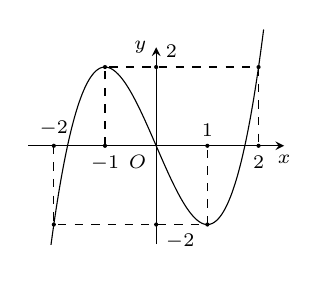
\begin{tikzpicture}[>=stealth,font=\scriptsize,x=1.3cm]
            \begin{scope}[scale=.5]
                \draw[->] (-2.5,0) -- (2.5,0) node[below] { $x$};
                \draw[->] (0,-2.5) -- (0,2.5) node[left] {$y$};
                \draw (0,0)node[below left]{ $O$};
                \draw (0,-2)node[below right]{$-2$} (0,2)node[above right]{\scriptsize $2$} (1,0) node[above]{ $1$} (-2,0) node[above]{ $-2$} (-1,0) node[below]{ $-1$} (2,0) node[below]{$2$};
                \draw[dashed] (-2,0)--(-2,-2)--(1,-2)--(1,0) (-1,0)--(-1,2)--(2,2)--(2,0);
                \clip (-2.5,-2.5)rectangle(2.5,3);
                \draw[samples=150,smooth,domain=-2.1:2.1] plot(\x,{(\x)^3-3*\x});

                \fill[black] (-2,0) circle(1.5pt) (-1,0) circle(1.5pt) (1,0) circle(1.5pt) (2,0) circle(1.5pt)(-2,-2) circle(1.5pt)(0,-2) circle(1.5pt)(1,-2) circle(1.5pt)(-1,2) circle(1.5pt)(0,2) circle(1.5pt)(2,2) circle(1.5pt);
            \end{scope}
    \end{tikzpicture}}
    \loigiai{
        Ta có $g'(x)=f'(2\cos x)\cdot(-2\sin x)-2\sin{2x}\cdot2=-2\sin{x}\left[f'(2\cos x)+4\cos x\right]$.\\
        Suy ra $g'(x)=0 \Leftrightarrow \hoac{&\sin x=0\\&f'(2\cos x)=-4\cos x.}$\\
        \begin{itemize}
            \item $\sin x=0 \Leftrightarrow x\in\{0;\pi\}$ vì $x\in(-\pi;2\pi)$.
            \item $f'(2\cos x)=-4\cos x$.\\
            Đặt $t=2\cos x$, vì $x\in(-\pi;2\pi)$ nên $t\in(-1;1)$.\\
            Phương trình trở thành $f'(t)=-2t$. Nghiệm của phương trình này là hoành độ giao điểm của đồ thị hàm số $y=f'(t)$ và đường thẳng $y=-2t$.\\
            \begin{center}
                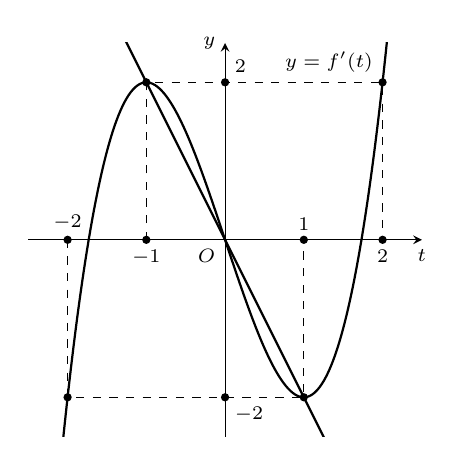
\begin{tikzpicture}[>=stealth,x=1cm,y=1cm,scale=1]
                    \draw[->] (-2.5,0) -- (2.5,0) node[below] {\scriptsize $t$};
                    \draw[->] (0,-2.5) -- (0,2.5) node[left] {\scriptsize $y$};
                    \draw (0,0)node[below left]{\scriptsize $O$};
                    \draw (0,-2)node[below right]{\scriptsize $-2$} (0,2)node[above right]{\scriptsize $2$} (1,0) node[above]{\scriptsize $1$} (-2,0) node[above]{\scriptsize $-2$} (-1,0) node[below]{\scriptsize $-1$} (2,0) node[below]{\scriptsize $2$};
                    \draw[dashed] (-2,0)--(-2,-2)--(1,-2)--(1,0) (-1,0)--(-1,2)--(2,2)--(2,0);
                    \clip (-2.5,-2.5)rectangle(2.5,2.5);
                    \draw[thick,samples=150,smooth,domain=-2.1:2.1] plot(\x,{(\x)^3-3*\x}) node[right]{$(l)$};
                    \node[above left] at (2,2){\scriptsize $y=f'(t)$};
                    \fill[black] (-2,0) circle(1.5pt) (-1,0) circle(1.5pt) (1,0) circle(1.5pt) (2,0) circle(1.5pt)(-2,-2) circle(1.5pt)(0,-2) circle(1.5pt)(1,-2) circle(1.5pt)(-1,2) circle(1.5pt)(0,2) circle(1.5pt)(2,2) circle(1.5pt);
                    \draw[thick,samples=150,smooth,domain=-2.1:2.1] plot(\x,{-2*(\x)});
                \end{tikzpicture}
            \end{center}
            Suy ra $f'(t)=-2t \Leftrightarrow \hoac{&t=-1\\&t=0\\&t=1.}$

            \begin{itemize}
                \item Với $t=-1 \Rightarrow 2\cos x=-1 \Leftrightarrow \cos x=-\dfrac{1}{2} \Leftrightarrow x\in\left\{-\dfrac{2\pi}{3};\dfrac{2\pi}{3};\dfrac{4\pi}{3}
                \right\}$ vì $x\in(-\pi;2\pi)$.
                \item Với $t=0 \Rightarrow \cos x=0 \Leftrightarrow x\in\left\{-\dfrac{\pi}{2};\dfrac{\pi}{2};\dfrac{3\pi}{2}
                \right\}$ vì $x\in(-\pi;2\pi)$.
                \item Với $t=1 \Rightarrow 2\cos x=1 \Leftrightarrow \cos x=\dfrac{1}{2} \Leftrightarrow x\in\left\{-\dfrac{\pi}{3};\dfrac{\pi}{3};\dfrac{5\pi}{3}
                \right\}$ vì $x\in(-\pi;2\pi)$.
            \end{itemize}
        \end{itemize}
        Và
        \begin{itemize}
            \item $f'(t)+2t>0\Leftrightarrow f'(t)>-2t\Leftrightarrow \hoac{&-1<t<0\\&t>1}\\
            \Rightarrow \hoac{&-\dfrac{1}{2}<\cos x<0\\&\cos x>\dfrac{1}{2}}\Leftrightarrow \hoac{&-\dfrac{2\pi}{3}<x<-\dfrac{\pi}{3}\\&\dfrac{4\pi}{3}<x<\dfrac{5\pi}{3}\\&\dfrac{\pi}{3}<x<\dfrac{2\pi}{3}}$ (vì $x\in(-\pi;2\pi)$).
            \item $f'(t)+2t<0\Leftrightarrow f'(t)<-2t\Leftrightarrow \hoac{&t<-1\\&0<t<1}\\
            \Rightarrow \hoac{&\cos x<-\dfrac{1}{2}\\&0<\cos x<\dfrac{1}{2}} \Leftrightarrow \hoac{&-\pi<x<-\dfrac{2\pi}{3}\\&-\dfrac{\pi}{3}<x<\dfrac{\pi}{3}\\&\dfrac{2\pi}{3}<x<\dfrac{4\pi}{3}}$ (vì $x\in(-\pi;2\pi)$).
        \end{itemize}
        Bảng biến thiên hàm số $y=g(x)$
        \begin{center}
            \begin{tikzpicture}
                \tkzTabInit[nocadre=false,lgt=4,espcl=1]
                {$x$ /1.1,$-2\sin x$ /0.7,$f'(2\cos x)+4\cos x$ /0.7,$g'(x)$ /0.7,$g(x)$ /2}
                {$-\pi$,$-\dfrac{2\pi}{3}$,$-\dfrac{\pi}{2}$,$-\dfrac{\pi}{3}$,$0$,$\dfrac{\pi}{3}$,$\dfrac{\pi}{2}$,$\dfrac{2\pi}{3}$,$\pi$,$\dfrac{4\pi}{3}$,$\dfrac{3\pi}{2}$,$\dfrac{5\pi}{3}$,$2\pi$}
                \tkzTabLine{,+,|,+,|,+,|,+,$0$,-,|,-,|,-,|,-,$0$,+,|,+,|,+,|,+,}
                \tkzTabLine{,-,$0$,+,$0$,-,$0$,+,|,+,$0$,-,$0$,+,$0$,-,|,-,$0$,+,$0$,-,$0$,+,}
                \tkzTabLine{,-,$0$,+,$0$,-,$0$,+,|,-,$0$,+,$0$,-,$0$,+,|,-,$0$,+,$0$,-,$0$,+,}
                \tkzTabVar{+/,-/,+/,-/,+/,-/,+/,-/,+/,-/,+/,-/,+/,}
            \end{tikzpicture}
        \end{center}
        Từ bảng biến thiên ta suy ra hàm số $y=g(x)$ có $11$ điểm cực trị trên khoảng $(-\pi;2\pi)$.
    }
\end{ex}
\begin{ex}%[2D1G2-6]
    \immini{	Cho hàm số $y=f(x)$ có đồ thị của $y=f'(x)$ có đồ thị như hình vẽ bên dưới. Hàm số $g(x)=f(x^3-3x)-x^3+3x$ có bao nhiêu điểm cực tiểu? \choice[2]
        {$2$}
        {$4$}
        {$3$}
        {\True $5$}}{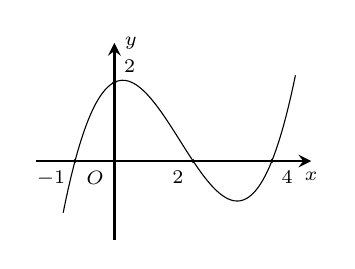
\begin{tikzpicture}[>=stealth,font=\scriptsize]
            \begin{scope}[scale=.5]
                \draw[->,line width = 1pt] (-2,0)--(0,0) node[below left]{$O$}--(5,0) node[below]{$x$};
                \draw[->,line width = 1pt] (0,-2) --(0,3) node[right]{$y$};
                \draw (-1,0) node[below left]{$-1$} circle (1pt);
                \draw (0,2) node[above right]{$2$} circle (1pt);
                \draw (2,0) node[below left]{$2$} circle (1pt);
                \draw (4,0) node[below right]{$4$} circle (1pt);
                \draw [ domain=-1.3:4.6, samples=100] %
                plot (\x, {0.25*(\x)^3-1.25*(\x)^2+0.5*(\x)+2});
            \end{scope}
    \end{tikzpicture}}
    \loigiai{
        $g'(x)=f'(x^3-3x)\cdot (3x^2-3)-3x^2+3=3(x^2-1)\left[f'(x^3-3x)-1\right].\\
        \Rightarrow g'(x)=0\Leftrightarrow \hoac{&x^2=1\\&f'(x^2-3x)=1} \Leftrightarrow \hoac{&x=\pm1\\&x^3-3x=a\quad (-1<a<0)\\&x^3-3x=b\quad (0<b<2)\\&x^3-3x=c\quad (c>4).}$\\
        \begin{center}
            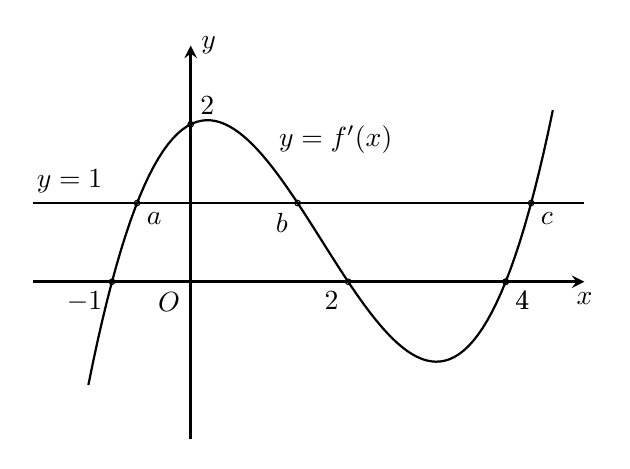
\begin{tikzpicture}[>=stealth]
                \draw[->,line width = 1pt] (-2,0)--(0,0) node[below left]{$O$}--(5,0) node[below]{$x$};
                \draw[->,line width = 1pt] (0,-2) --(0,3) node[right]{$y$};
                \draw (-1,0) node[below left]{$-1$} circle (1pt);
                \draw (0,2) node[above right]{$2$} circle (1pt);
                \draw (2,0) node[below left]{$2$} circle (1pt);
                \draw (4,0) node[below right]{$4$} circle (1pt);
                \draw [thick, domain=-1.3:4.6, samples=100] %
                plot (\x, {0.25*(\x)^3-1.25*(\x)^2+0.5*(\x)+2});
                \draw [thick, domain=-2:5, samples=100] %
                plot (\x, {0*(\x)+1});
                \draw (-1,1) node[above left]{$y=1$};
                \draw (1,1.8) node[right]{$y=f'(x)$};
                \draw (4,0) node[below right]{$4$} circle(1pt);
                \draw (4.323404276086477,1) node[below right] {$c$} circle(1pt);
                \draw (1.3579263675184994,1) node[below left] {$b$} circle(1pt);
                \draw (-0.6813306436049771,1) node[below right] {$a$} circle(1pt);
            \end{tikzpicture}
        \end{center}
        \begin{itemize}
            \item Phương trình $x^3-3x=a$ có $3$ nghiệm $x_1$, $x_2$, $x_3$ với $x_1<x_2<x_3$.
            \item Phương trình $x^3-3x=b$ có $3$ nghiệm $x_4$, $x_5$, $x_6$ với $x_4<x_5<x_6$.
            \item Phương trình $x^3-3x=c$ có $1$ nghiệm $x_7\quad(x_7>x_6)$.
        \end{itemize}
        \begin{center}
            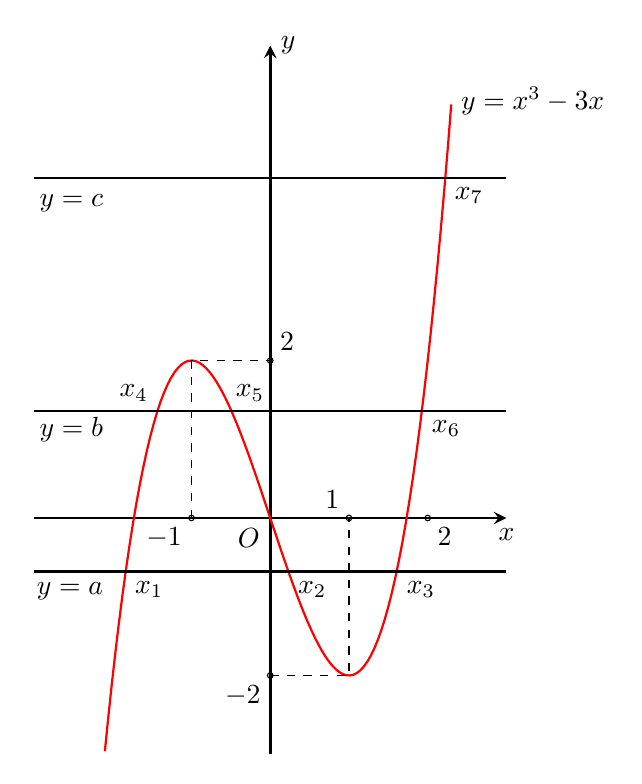
\begin{tikzpicture}[>=stealth]
                \draw[->,line width = 1pt] (-3,0)--(0,0) node[below left]{$O$}--(3,0) node[below]{$x$};
                \draw[->,line width = 1pt] (0,-3) --(0,6) node[right]{$y$};
                \draw (-1,0) node[below left]{$-1$} circle (1pt);
                \draw (0,2) node[above right]{$2$} circle (1pt);
                \draw (1,0) node[above left]{$1$} circle (1pt);
                \draw (2,0) node[below right]{$2$} circle (1pt);
                \draw (0,-2) node[below left]{$-2$} circle (1pt);
                \draw [thick,color=red, domain=-2.1:2.3, samples=100] %
                plot (\x, {(\x)^3-3*(\x)});
                \draw [thick, domain=-3:3, samples=100] plot (\x, {0*(\x)+4.32});
                \draw [thick, domain=-3:3, samples=100] plot (\x, {0*(\x)+1.36});
                \draw [thick, domain=-3:3, samples=100] plot (\x, {0*(\x)-0.68});
                \draw (2.3,5) node[above right]{$y=x^3-3x$};
                \draw (-2,-0.7) node[below left]{$y=a$};
                \draw (-2,1.4) node[below left]{$y=b$};
                \draw (-2,4) node[left]{$y=c$};
                \draw[dashed](-1,0)--(-1,2)--(0,2);
                \draw[dashed](0,-2)--(1,-2)--(1,0);
                \draw (-1.84,-0.68) node[below right] {$x_1$};
                \draw (0.23,-0.68) node[below right] {$x_2$};
                \draw (1.61,-0.68) node[below right] {$x_3$};
                \draw (-1.43,1.36) node[above left] {$x_4$};
                \draw (-0.56,1.36) node[above right] {$x_5$};
                \draw (1.93,1.36) node[below right] {$x_6$};
                \draw (2.22,4.32) node[below right] {$x_7$};
            \end{tikzpicture}
        \end{center}
        Bảng xét dấu $g'(x)$
        \begin{center}
            
\begin{tikzpicture}
                \tkzTabInit[nocadre=false,lgt=2.3,espcl=1.3]
                {$x$ /1.1,$x^2-1$ /0.7,$f'(x^3-3x)$ /0.7,$g'(x)$ /0.7,$g(x)$ /2}
                {$-\infty$,$x_1$,$x_4$,$-1$,$x_5$,$x_2$,$1$,$x_3$,$x_6$,$x_7$,$+\infty$}
                \tkzTabLine{,+,|,+,|,+,$0$,-,|,-,|,-,$0$,+,|,+,|,+,|,+,}
                \tkzTabLine{,-,$0$,+,$0$,-,|,-,$0$,+,$0$,-,|,-,$0$,+,$0$,-,$0$,+,}
                \tkzTabLine{,-,$0$,+,$0$,-,$0$,+,$0$,-,$0$,+,$0$,-,$0$,+,$0$,-,$0$,+,}
                \tkzTabVar{+/,-/,+/,-/,+/,-/,+/,-/,+/,-/,+/}
            \end{tikzpicture}
        \end{center}
        Dựa vào bảng xét dấu ta kết luận hàm số $y=g(x)$ có $5$ điểm cực tiểu.
    }
\end{ex}
\begin{ex}%[2D1G2-2]
    \immini{Cho hàm số $y=f(x)$ có đạo hàm và liên tục trên $\mathbb{R}$ và có đồ thị $y=f'(x)$ như hình vẽ. Hàm $y=f(x^2-2)-\dfrac{1}{2}x^4+\dfrac{3}{2}x^2$ có bao nhiêu điểm cực tiểu?
        \choice[2]
        {$4$}
        {$1$}
        {$2$}
        {\True$3$}}
    {\begin{tikzpicture}[>=stealth,font=\scriptsize,x=1.2cm]
            \begin{scope}[scale=.7]
                \def\mx{-1} \def\max{3}
                \def\my{-1} \def\may{3.5}
                \def\hamso(#1,#2){plot [samples=200,smooth,domain=#1:#2](\x,{
                        2*(\x)^4-5*(\x)^3+1.5*(\x)^2+2.25*(\x)
                    })}
                \draw[fill=black]
                (-0.5,0)circle (.7pt)node[shift={(-110:.5)}]{$-\dfrac{1}{2}$}
                (0.5,0)circle (.7pt)node[shift={(-90:.5)}]{$\dfrac{1}{2}$}
                (2,0)circle (.7pt)node[shift={(-90:.5)}]{$2$}
                (1.5,0)circle (.7pt)node[shift={(-90:.5)}]{$\dfrac{3}{2}$}
                (0,1)circle (.7pt)node[shift={(180:.3)}]{$1$}
                (0,2.5)circle (.7pt)node[shift={(180:.3)}]{$\dfrac{5}{2}$}
                (0.5,1)circle (.7pt)
                (2,2.5)circle (.7pt)
                ;
                \draw[dashed,thin] (0.5,0)|-(0,1)(2,0)|-(0,2.5);
                %===========================================
                \draw[->] (\mx,0)--(0,0) node [below right] {$O$}--(\max,0) node[below] {$x$};
                \draw[->] (0,\my)--(0,\may) node[left] {$y$};
                \clip (\mx,\my) rectangle (\max,\may);
                \draw \hamso(\mx,\max);
            \end{scope}
    \end{tikzpicture}}
    \loigiai{
        \immini{
            Ta có $y'=2xf'(x^2-2)-2x^3+3x=2x\left(f'(x^2-2)-x^2+\dfrac{3}{2}\right)$.\\
            $y'=0\Leftrightarrow \hoac{&x=0\\&f'(x^2-2)-x^2+\dfrac{3}{2}=0.\quad(*)}$\\
            Đặt $t=x^2-2$ ta có $(*)\Leftrightarrow f'(t)-t-\dfrac{1}{2}=0\Leftrightarrow f'(t)=t+\dfrac{1}{2}$.\\
            Dựa vào đồ thị hàm số bên ta có
            $$f'(t)=t+\dfrac{1}{2}\Leftrightarrow \hoac{&t=-\dfrac{1}{2}\\&t=\dfrac{1}{2}\\&t=2.}$$
        }{
            \begin{tikzpicture}[scale=1.2,>=stealth,font=\footnotesize,y=.8cm]
                \def\mx{-1} \def\max{3}
                \def\my{-1} \def\may{3.5}
                \def\hamso(#1,#2){plot [samples=200,smooth,domain=#1:#2](\x,{
                        (\x)+0.5
                    })}
                \def\ham(#1,#2){plot [samples=200,smooth,domain=#1:#2](\x,{
                        2*(\x)^4-5*(\x)^3+1.5*(\x)^2+2.25*(\x)
                    })}
                \draw[fill=black]
                (-0.5,0)circle (.7pt)node[shift={(-110:.5)}]{$-\dfrac{1}{2}$}
                (0.5,0)circle (.7pt)node[shift={(-90:.5)}]{$\dfrac{1}{2}$}
                (2,0)circle (.7pt)node[shift={(-90:.5)}]{$2$}
                (1.5,0)circle (.7pt)node[shift={(-90:.5)}]{$\dfrac{3}{2}$}
                (0,1)circle (.7pt)node[shift={(180:.3)}]{$1$}
                (0,2.5)circle (.7pt)node[shift={(180:.3)}]{$\dfrac{5}{2}$}
                (0.5,1)circle (.7pt)
                (2,2.5)circle (.7pt)
                ;
                \draw[dashed,thin] (0.5,0)|-(0,1)(2,0)|-(0,2.5);
                %===========================================
                \draw[->] (\mx,0)--(0,0) node [below right] {$O$}--(\max,0) node[below] {$t$};
                \draw[->] (0,\my)--(0,\may) node[left] {$y$};
                \clip (\mx,\my) rectangle (\max,\may);
                \draw \hamso(\mx,\max)\ham(\mx,\max);
        \end{tikzpicture}}
        \noindent
        Suy ra $\hoac{&x^2-2=-\dfrac{1}{2}\\&x^2-2=\dfrac{1}{2}\\&x^2-2=2}\Leftrightarrow\hoac{&x=\pm\dfrac{\sqrt{6}}{2}\\&x=\pm\dfrac{\sqrt{10}}{2} &\text{ (nghiệm kép)}\\&x=\pm 2.}$\\
        Bảng xét dấu
        \begin{center}
            
\begin{tikzpicture}
                \tkzTabInit[nocadre=false, lgt=0.7,espcl=1.6,deltacl=0.5]
                {$x$/1.2, $y'$ /0.6}
                {$-\infty$ , $-2$ , $-\dfrac{\sqrt{10}}{2}$ ,$-\dfrac{\sqrt{6}}{2}$,$0$,$\dfrac{\sqrt{6}}{2}$,$\dfrac{\sqrt{10}}{2}$ ,$2$, $+\infty$}
                \tkzTabLine{ ,-,0,+, 0 ,+, 0 ,-,0,+,0,-,0,-,0,+ }
            \end{tikzpicture}
        \end{center}
        Suy ra hàm số có $3$ điểm cực tiểu.
    }
\end{ex}
\begin{ex}%[2D1G2-6]
    \immini{Cho hàm số $y=f(x)$ có bảng biến thiên bên dưới. Số điểm cực đại và số điểm cực tiểu của hàm số $y=f^2(2x)-2f(2x)+1$ lần lượt là
        \choice
        {\True $2$ và $3$}
        {$3$ và $2$}
        {$1$ và $1$}
        {$2$ và $2$}}{
\begin{tikzpicture}
            \tkzTabInit[nocadre=false,lgt=1.2,espcl=2,deltacl=0.6]
            {$x$ /0.6,$f'(x)$ /0.6,$f(x)$ /2}
            {$-\infty$,$-1$,$2$,$+\infty$}
            \tkzTabLine{,-,$0$,+,$0$,-,}
            \tkzTabVar{+/$+\infty$,-/$0$,+/$3$,-/$-\infty$}
    \end{tikzpicture}}
    \loigiai{
        Đặt $g(x)=	f^2(2x)-2f(2x)+1=\left[f(2x)-1\right]^2$.\\
        $\Rightarrow g'(x)=2\cdot\left[f(2x)-1\right]\cdot f'(2x)$.\\
        $\Rightarrow g'(x)=0\Leftrightarrow \hoac{&f(2x)=1\\&f'(2x)=0.}$\\
        \begin{itemize}
            \item $f(2x)=1\Leftrightarrow \hoac{&2x=a\quad(a<-1)\\&2x=b\quad(-1<b<2)\\&2x=c\quad(2<c)}\Leftrightarrow \hoac{&x=\dfrac{a}{2}\quad(\dfrac{a}{2}<-\dfrac{1}{2})\\&x=\dfrac{b}{2}\quad(-\dfrac{1}{2}<\dfrac{b}{2}<1)\\&x=\dfrac{c}{2}\quad(1<\dfrac{c}{2}).}$
            \item $f'(2x)=0\Leftrightarrow\hoac{&2x=-1\\&2x=2}\Leftrightarrow\hoac{&x=-\dfrac{1}{2}\\&x=1.}$
        \end{itemize}
        Bảng biến thiên hàm số $y=g(x)$
        \begin{center}
            
\begin{tikzpicture}
                \tkzTabInit[nocadre=false,lgt=2.1,espcl=2,deltacl=0.6]
                {$x$ /1.1,$f'(2x)$ /0.7,$f(2x)-1$ /0.7,$g'(x)$ /0.7,$g(x)$ /2}
                {$-\infty$,$\dfrac{a}{2}$,$-\dfrac{1}{2}$,$\dfrac{b}{2}$,$1$,$\dfrac{c}{2}$,$+\infty$}
                \tkzTabLine{,-,|,-,$0$,+,|,+,$0$,-,|,-,}
                \tkzTabLine{,+,$0$,-,|,-,$0$,+,|,+,$0$,-,}
                \tkzTabLine{,-,$0$,+,$0$,-,$0$,+,$0$,-,$0$,+,}
                \tkzTabVar{+/,-/,+/,-/,+/,-/,+/}
            \end{tikzpicture}
        \end{center}
        Dựa vào bảng biến thiên ta thấy hàm số $y=g(x)$ có $2$ điểm cực đại và $3$ điểm cực tiểu.
    }
\end{ex}

\begin{ex}%[2D1G2-6]
    Cho hàm số bậc ba $y=f(x)$ có đồ thị như hình bên. Có bao nhiêu giá trị nguyên của tham số $m$ để hàm số $y=\vert f^2(x)+2f(x)+m\vert$ có $9$ điểm cực trị?
    \choice
    {\True $24$}
    {Vô số}
    {$25$}
    {$23$}
    \loigiai{
        Đặt $y=g(x)=f^2(x)+2f(x)+m=\left[f(x)+1\right]^2+m-1.\\
        \Rightarrow g'(x)=2\left[f(x)+1\right]\cdot f'(x).\\
        \Rightarrow g'(x)=0\Leftrightarrow \hoac{&f'(x)=0\\&f(x)=-1}\Leftrightarrow \hoac{&x=1\\&x=3\\&x=a\quad(0<a<1)\\&x=b\quad(1<b<3)\\&x=c\quad(3<c).}$\\
        Từ đồ thị ta suy ra
        \begin{itemize}
            \item $f'(x)+1>0\Leftrightarrow f'(x)>-1\Leftrightarrow a<x<b \text{ hoặc } x>c$.
            \item $f'(x)+1<0\Leftrightarrow f'(x)<-1\Leftrightarrow x<a \text{ hoặc } b<x<c$.
        \end{itemize}
        Bảng biến thiên hàm số $y=g(x)$
        \begin{center}
            
\begin{tikzpicture}
                \tkzTabInit[nocadre=false,lgt=2.3,espcl=1.8]
                {$x$ /1.1,$f'(x)$ /0.7,$f(x)+1$ /0.7,$g'(x)$ /0.7,$g(x)$ /2}
                {$-\infty$,$0$,$a$,$1$,$b$,$3$,$c$,$+\infty$}
                \tkzTabLine{,+,t,+,|,+,$0$,-,|,-,$0$,+,|,+,}
                \tkzTabLine{,-,t,-,$0$,+,|,+,$0$,-,|,-,$0$,+,}
                \tkzTabLine{,-,t,-,$0$,+,$0$,-,$0$,+,$0$,-,$0$,+,}
                \tkzTabVar{+/,R,-/$m-1$,+/$m+24$,-/$m-1$,+/$m$,-/$m-1$,+/}
            \end{tikzpicture}
        \end{center}
        Đồ thị hàm số $y=|g(x)|$ gồm có $2$ phần như sau:
        \begin{itemize}
            \item Phần 1: Trùng với đồ thị hàm số $y=g(x)$ với $g(x)\ge0$.
            \item Phần 2: Là phần đối xứng với phần đồ thị của hàm số $y=g(x)$ với $g(x)<0$ qua trục $\text{Ox}$.
        \end{itemize}
        Kết hợp với bảng biến thiên hàm số $y=g(x)$ ta suy ra hàm số $y=|g(x)|$ có $9$ điểm cực trị khi và chỉ khi $m\le 0<m+24 \Leftrightarrow -24<m\le0$. Mà $m$ là số nguyên nên ta được $24$ giá trị của $m$.
    }
\end{ex}
\begin{ex}%[2D1K2-6]
    Có bao giá trị nguyên của tham số $m$ thoả mãn $\vert m\vert<10$ sao cho hàm số $y=\vert x^3-(m-2)x^2-mx-m^2\vert$ có $3$ điểm cực tiểu?
    \choice
    {$9$}
    {$10$}
    {\True $8$}
    {$16$}
    \loigiai{
        Đặt hàm số $y=f(x)=x^3-(m-2)x^2-mx-m^2=(x-m)(x^2+2x+m)=(x-m)\left[x(x+2)+m\right]$.
        Suy ra $f'(x)=3x^2-2(m-2)x-m=0$ có $\Delta'=(m-2)^2+3m=m^2-m+4>0$ với mọi $m$.\\
        Theo định lí Vi-ét ta có $\heva{&x_1+x_2=\dfrac{2(m-2)}{3}\\&x_1x_2=-\dfrac{m}{3}}$.\\
        Hàm số $y=|f(x)|$ có $3$ điểm cực tiểu khi và chỉ khi $y(x_1)\cdot y(x_2)<0$.\\
        Thực hiện biến đổi\\
        $y(x_1)\cdot y(x_2)=  (x_1-m)(x_2-m)\left[x_1(x_1+2)+m\right]\left[x_2(x_2+2)+m\right]\\
        = (x_1-m)(x_2-m)\left[x_1x_2(x_1+2)(x_2+2)+m(x_1^2+x_2^2)+2m(x_1+x_2)+m^2\right]\\
        = \left[x_1x_2-m(x_1+x_2)+m^2\right]\left[x_1x_2\left(x_1x_2+2(x_1+x_2)+4\right)+m(x_1^2+x_2^2)+2m(x_1+x_2)+m^2\right]\\
        = \left(\dfrac{m^2}{3}+m\right)\left[-\dfrac{m}{3}\left(m+\dfrac{4}{3}\right)+m\left(\dfrac{4m^2}{9}-\dfrac{10m}{9}+\dfrac{16}{9}\right)+\dfrac{4m^2}{3}-\dfrac{8m}{3}+m^2\right]\\
        = \dfrac{2}{27}m^2(m+3)(2m^2+4m-5)$.\\
        Suy ra $y(x_1)\cdot y(x_2)<0\Leftrightarrow m^2(m+3)(2m^2+4m-5)<0\Leftrightarrow \hoac{&m<-3\\&\dfrac{-2-\sqrt{14}}{2}<m<0\\&0<m<\dfrac{-2+\sqrt{14}}{2}}$.\\
        Kết hợp với điều kiện $m$ là số nguyên thỏa $|m|<10$ ta được $m\in\{-9;-8;-7;-6;-5;-4;-2;-1\}$.\\
        Vậy có $8$ giá trị nguyên của tham số $m$.
    }
\end{ex}

\begin{ex}%[2D1G2-6]
    \immini{	Cho hàm số $f(x)=ax^4+bx^3+cx^2+dx+e, (ae<0)$. Đồ thì hàm số $y=f'(x)$ như hình bên dưới. Hàm số $y=\left|4f(x)-x^2\right|$ có bao nhiêu điểm cực tiểu?
        \choice[2]
        {$4$}
        {$5$}
        {\True $3$}
        {$2$}
    }{\begin{tikzpicture}[>=stealth,font=\scriptsize,x=1.3cm,y=1.5cm]
            \begin{scope}[scale=0.5]
                \draw[->] (-2,0) -- (3,0) node[below] { $x$};
                \draw[->] (0,-1) -- (0,3) node[left] {\ $y$};
                \draw (0,0) node[above left] { $O$} circle (1pt);
                \draw[smooth](0,0) parabola bend (-0.6,-1)(-1.7,1.7);
                \draw(0,0) parabola bend (1.3,2.5)(2,1);
                \draw [dashed] (0,1)--(2,1)--(2,0);
                \draw [dashed] (-1.05,0)--(-1.05,-0.5)--(0,-0.5);
                \draw (-1,0) node[above] { $-1$};
                \draw (0,-0.5) node[right] { $-\dfrac{1}{2}$};
                \draw (0,1) node[left] { $1$};
                \draw (2,0) node[below] { $2$};
            \end{scope}
    \end{tikzpicture}}
    \loigiai{
        Ta có $f'(x)=4ax^3+3bx^2+2cx+d$. Từ đồ thị hàm số $f'(x)$ suy ra $a<0$, do đó $e>0$.\\
        Đặt $y=g(x)=4f(x)-x^2\Rightarrow g'(x)	=4f'(x)-2x=4\left[f'(x)-\dfrac{x}{2}\right]$.\\
        \begin{center}
            \begin{tikzpicture}[>=stealth,x=1.0cm,y=1.0cm,thick, scale=1.0]
                \draw[->] (-2,0) -- (3,0) node[below] {\footnotesize $x$};
                \draw[->] (0,-1) -- (0,3) node[left] {\footnotesize $y$};
                \draw (0,0) node[below left] {\footnotesize $O$} circle (1pt);
                \draw[smooth](0,0) parabola bend (-0.6,-1)(-1.7,1.7);
                \draw(0,0) parabola bend (1.3,2.5)(2,1);
                \draw [dashed] (0,1)--(2,1)--(2,0);
                \draw [dashed] (-1.05,0)--(-1.05,-0.5)--(0,-0.5);
                \draw (-1,0) node[above] {\footnotesize $-1$};
                \draw (0,-0.5) node[right] {\footnotesize $-\dfrac{1}{2}$};
                \draw (0,1) node[left] {\footnotesize $1$};
                \draw (2,0) node[below] {\footnotesize $2$};
                \draw [thick, domain=-2.1:2.5, samples=100] %
                plot (\x, {0.5*(\x)});
            \end{tikzpicture}
        \end{center}
        Suy ra $g'(x)=0\Leftrightarrow f'(x)-\dfrac{x}{2}=0\Leftrightarrow f'(x)=\dfrac{x}{2}\Leftrightarrow \hoac{&x=-1\\&x=0\\&x=2}$.\\
        Bảng biến thiên
        \begin{center}
            
\begin{tikzpicture}
                \tkzTabInit[nocadre=false,lgt=1.2,espcl=2.3]
                {$x$ /0.6,$g'(x)$ /0.6,$g(x)$ /2}
                {$-\infty$,$-1$,$0$,$2$,$+\infty$}
                \tkzTabLine{,+,$0$,-,$0$,+,$0$,-,}
                \tkzTabVar{-/,+/,-/$4e$,+/,-/}
            \end{tikzpicture}
        \end{center}
        Vì $4e>0$ nên từ bảng biến thiên hàm số $g(x)$ ta suy ra hàm số $y=\left|g(x)\right|$ có $3$ điểm cực tiểu.
    }
\end{ex}

\begin{ex}%[2D1G2-6]
    \immini{	Cho hàm số bậc bốn $f(x)$ có $f(0)=-1$. Hàm số $y=f'(x)$ có đồ thị là hình bên. Số điểm cực trị của hàm số $y=\vert 4f(x+1)+x^2+2x\vert$ là
        \choice[2]
        {$3$}
        {\True $5$}
        {$4$}
        {$6$}}{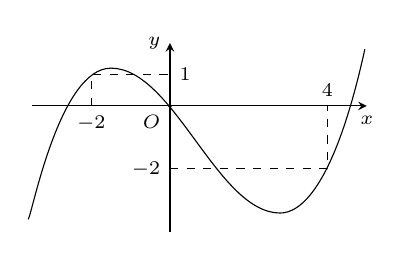
\begin{tikzpicture}[>=stealth,font=\scriptsize,y=.8cm]
            \begin{scope}[scale=.5]
                \draw[->] (-3.5,0) -- (5,0) node[below] {$x$};
                \draw[->] (0,-4) -- (0,2) node[left] { $y$};
                \draw (0,0) node[below left] {$O$} circle (1pt);
                \draw (-3.6,-3.6) ..controls +(60:0.2) and +(-180:1.3).. (-1.5,1.2) ..controls +(0:1.6) and +(-180:1.6) .. (2.8,-3.4)..controls +(0:0.5) and +(-100:4.5) .. (4.95,1.8);
                \draw [dashed] (-2,0)--(-2,1)--(0,1);
                \draw [dashed] (0,-2)--(4,-2)--(4,0);
                \draw (-2,0) node[below] { $-2$};
                \draw (0,-2) node[left] { $-2$};
                \draw (0,1) node[right] { $1$};
                \draw (4,0) node[above] {$4$};
            \end{scope}
    \end{tikzpicture}}
    \loigiai{
        Đặt $y=g(x)=4f(x+1)+x^2+2x\Rightarrow g'(x)=4f'(x+1)+2x+2=4\left[f'(x+1)+\dfrac{x+1}{2}\right]$.\\
        Suy ra $g'(x)=0\Leftrightarrow f'(x+1)=-\dfrac{x+1}{2}$.\\
        Đặt $t=x+1$ thì phương trình trở thành $f'(t)=-\dfrac{t}{2}$. Nghiệm của phương trình này là hoành độ giao điểm của đồ thị hàm số $y=f'(t)$ và $y=-\dfrac{t}{2}$.
        \begin{center}
            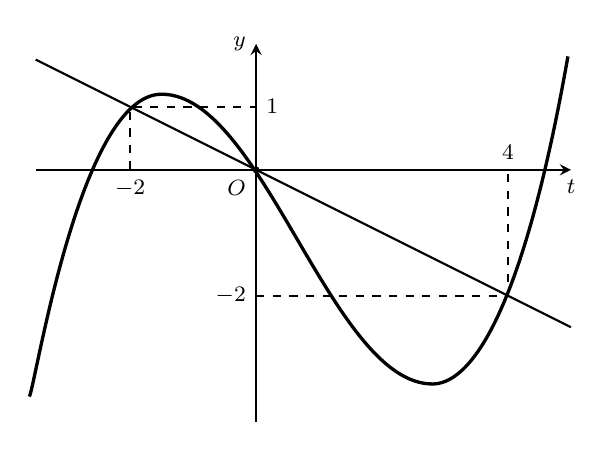
\begin{tikzpicture}[>=stealth,x=1.0cm,y=1.0cm,thick, scale=0.8]
                \draw[->] (-3.5,0) -- (5,0) node[below] {\footnotesize $t$};
                \draw[->] (0,-4) -- (0,2) node[left] {\footnotesize $y$};
                \draw (0,0) node[below left] {\footnotesize $O$} circle (1pt);
                \draw[very thick] (-3.6,-3.6) ..controls +(60:0.2) and +(-180:1.3).. (-1.5,1.2) ..controls +(0:1.6) and +(-180:1.6) .. (2.8,-3.4)..controls +(0:0.5) and +(-100:4.5) .. (4.95,1.8);
                \draw [thick, domain=-3.5:5, samples=100] %
                plot (\x, {-0.5*(\x)});
                \draw [dashed] (-2,0)--(-2,1)--(0,1);
                \draw [dashed] (0,-2)--(4,-2)--(4,0);
                \draw (-2,0) node[below] {\footnotesize $-2$};
                \draw (0,-2) node[left] {\footnotesize $-2$};
                \draw (0,1) node[right] {\footnotesize $1$};
                \draw (4,0) node[above] {\footnotesize $4$};
            \end{tikzpicture}
        \end{center}
        Do đó\\
        $$f'(t)=-\dfrac{t}{2}\Leftrightarrow\hoac{&t=-2\\&t=0\\&t=4}\Rightarrow \hoac{&x+1=-2\\&x+1=0\\&x+1=4}\Leftrightarrow \hoac{&x=-3\\&x=-1\\&x=3.}$$
        Bảng biến thiên
        \begin{center}
            
\begin{tikzpicture}
                \tkzTabInit[nocadre=false,lgt=1.2,espcl=2.3]
                {$x$ /0.6,$g'(x)$ /0.6,$g(x)$ /2}
                {$-\infty$,$-3$,$-1$,$3$,$+\infty$}
                \tkzTabLine{,-,$0$,+,$0$,-,$0$,+,}
                \tkzTabVar{+/,-/,+/$-5$,-/,+/}
            \end{tikzpicture}
        \end{center}
        Từ bảng biến thiên suy ra hàm số $y=g(x)$ có $3$ cực trị âm, do đó hàm số $y=\left|g(x)\right|$ có $5$ điểm cực trị.
    }
\end{ex}
\begin{ex}%[2D1Y2-6]
    \immini{	Cho hàm số $y=f(x)$ có bảng biến thiên như hình vẽ. Hàm số $y=f\left(|x|\right)$ đạt cực đại tại.
        \choice[2]
        {$x=-1$}
        {\True $x=0$}
        {$x=2$}
        {$x=-2$}}{
\begin{tikzpicture}[>=stealth,scale=0.9]
            \tkzTabInit[nocadre=false,lgt=1,espcl=2.6,deltacl=0.5]{$x$/.7 ,$y'$/.7,$y$/2}
            {$-\infty$ , $-1$ , $2$ , $+\infty$}
            \tkzTabLine{ , + , $0$ , - , $0$ , + , }
            \tkzTabVar{-/$-\infty$ , +/$3$ , -/$1$ , +/$+\infty$}
    \end{tikzpicture}}
    \loigiai{Từ bảng biến thiên của hàm số $y=f(x)$ ta có bảng biến thiên của hàm số $y=f\left(|x|\right)$ như sau
        \begin{center}
            \begin{tikzpicture}[scale=0.9]
                \foreach \x/\texn in {0/x,2/-\infty,4/-2,6/0,8/2,10/+\infty} \path (\x,3.5)node{$\texn$};
                \foreach \x/\texn in
                {0/y',3/-,4/0,5/+,6/0,7/-,8/0,9/+} \path (\x,2.5)node{$\texn$};
                \foreach \x/\y/\texn in {0/1/y,
                    2/1.5/+\infty,4/0/1,6/1.0/f(0),8/0/1,10/1.5/+\infty}
                \path (\x,\y) node(\x){$\texn$};
                \foreach \x/\y/\texn in {2/4,4/6,6/8,8/10}
                \draw[-stealth] (\x)--(\y);
                \draw
                (-.5,3)--(10.5,3) (1,4)--(1,0)
                (-.5,2)--(10.5,2);
            \end{tikzpicture}
        \end{center}
        Từ bảng biến thiên ta thấy hàm số $y=f\left(|x|\right)$ đạt cực đại tại $x=0$.
    }
\end{ex}
%%=====Câu 70
\begin{ex}%[2D1Y2-6]
    \immini{	Cho hàm số $y=f(x)$ có bảng biến thiên như hình vẽ. Tổng các giá trị cực đại của hàm số $y=\left|f(x)\right|$ là
        \choice[2]
        {\True $9$}
        {$-3$}
        {$3$}
        {$7$}}{\begin{tikzpicture}[>=stealth]
            \tkzTabInit[nocadre=false,lgt=1,espcl=1.7,deltacl=0.5]{$x$/.7 ,$y'$/.7,$y$/2}
            {$-\infty$ , $-1$ , $0$ , $1$ , $+\infty$}
            \tkzTabLine{ , - , $0$ , + , $0$ , - , $0$ , + , }
            \tkzTabVar{+/$+\infty$ , -/$-2$, +/$3$ , -/$-4$ , +/$+\infty$}
    \end{tikzpicture}}
    \loigiai{Từ bảng biến thiên của hàm số $y=f(x)$ ta có bảng biến thiên của hàm số $y=\left|f(x)\right|$ như sau
        \begin{center}
            \begin{tikzpicture}[scale=0.8]
                \foreach \x/\texn in {0/x,2/-\infty,4/x_1,6/-1,8/x_2,10/0,12/x_3,14/1,16/x_4,18/+\infty} \path (\x,3.5)node{$\texn$};
                \foreach \x/\texn in
                {0/y',3/-,4/||,5/+,6/0,7/-,8/||,9/+,10/0,11/-,12/||,13/+,14/0,15/-,16/||,17/+} \path (\x,2.5)node{$\texn$};
                \foreach \x/\y/\texn in {0/1/y,
                    2/1.5/+\infty,4/0/0,6/0.5/2,8/0/0,10/0.7/3,12/0/0,14/1.0/4,16/0/0,18/1.5/+\infty}
                \path (\x,\y) node(\x){$\texn$};
                \foreach \x/\y/\texn in {2/4,4/6,6/8,8/10,10/12,12/14,14/16,16/18}
                \draw[-stealth] (\x)--(\y);
                \foreach \x in {4,8,12}\draw[dashed,red] (\x)--+(3.7,0);
                \draw[dashed,red] (1.2,0)--+(2.7,0) (16)--+(2.0,0) node[below=-.1]{\small $y=0$};
                \draw
                (-.5,3)--(18.5,3) (1,4)--(1,0)
                (-.5,2)--(18.5,2);
            \end{tikzpicture}
        \end{center}
        Từ bảng biến thiên ta thấy hàm số $y=\left|f(x)\right|$ có $3$ giá trị cực đại lần lượt là $2$, $3$, $4$.\\
        Tổng các giá trị cực đại là $9$.
    }
\end{ex}
\begin{ex}%[2D1Y2-6]
    Cho hàm số $y=f(x)$ có đạo hàm $y=f'(x)=(x-1)(x-2)^4(x^2-4)$. Số điểm cực trị của hàm số $y=f(|x|)$ là
    \choice
    {$3$}
    {$2$}
    {$4$}
    {\True $5$}
\end{ex}
\begin{ex}%[2D1Y2-6]
    Cho hàm số $y=f(x)$ có đạo hàm $y=f'(x)=(x^3-2x^2)(x^3-2x)$ trên $\mathbb{R}$. Hàm số $y=|f(4-2021x)|$ có nhiều nhất bao nhiêu điểm cực trị?
    \choice
    {\True$9$}
    {$11$}
    {$2021$}
    { $5$}
\end{ex}
\begin{ex}%[2D1B2-6]
    Có bao nhiêu giá trị nguyên của tham số $m$ để hàm số $y=|3x^4-4x^3-12x^2+m|$ có $7$ điểm cực trị?
    \choice
    {$3$}
    {$5$}
    {$6$}
    {\True $4$}
    \loigiai{
        Đặt $f(x)=3x^4-4x^3-12x^2+m$ $\Rightarrow f'(x)=12x^3-12x^2-24x=0 \Rightarrow x=0; x=-1; x=2$.\\
        Qua BBT của $y=f(x)$ ta suy ra $y=|f(x)|$ có $7$ điểm cực trị $\Rightarrow \heva{&m>0\\&m-5<0} \Rightarrow 0<m<5$. Vậy có $4$ giá trị nguyên $m$ thỏa yêu cầu bài toán.
    }
\end{ex}
\begin{ex}%[2D1B2-6]
    Tìm các giá trị của $m$ để hàm số $f(x)=|x^3+3x^2+m-3|$ có ba điểm cực trị.
    \choice
    {$m=3; m=-1$}
    {$m\ge 1; m \le-3$}
    {$1\le m \le 3$}
    {\True $m\ge 3; m \le -1$}
\end{ex}
\begin{ex}%[2D1B2-6]
    Cho hàm số $y=f(x)=x^3-3mx^2+3(m^2-4)x+1$, có bao nhiêu số nguyên $m \in (-10;10)$  để hàm số $y=f(|x|)$ có đúng $5$ điểm cực trị.
    \choice
    {$3$}
    {$6$}
    {$8$}
    {\True $7$}
    \loigiai{
        $y=f(|x|)$ có đúng $5$ điểm cực trị $\Rightarrow y=f(x)$ có hai điểm cực trị dương.\\
        $f'(x)=3x^2-6mx+3(m^2-4)=0 \Rightarrow x=m-2; x=m+2$ có hai nghiệm dương $\Leftrightarrow m-2>0 \Leftrightarrow m >2$.\\ Vậy có $7$ giá trị $m$ thỏa yêu cầu bài toán.
    }
\end{ex}
\begin{ex}%[2D1G2-6]
    Cho hàm số $f(x)=\dfrac{1}{3}x^3-(2m-1)x^2+(8-m)x+2020$ với $m$ là tham số. Tập hợp tất cả các giá trị của tham số $m$ để hàm số $y=f\left(\vert x\vert\right)$ có điểm $5$ cực trị là khoảng $(a;b)$. Tích $a\cdot b$ bằng
    \choice
    {$12$}
    {$16$}
    {$10$}
    {\True $14$}
    \loigiai{
        Tập xác định $\mathscr{D}=\mathbb{R}$.\\
        Ta có $f\left(|-x|\right)=f\left(|x|\right)$, $\forall x\in\mathbb{R}$ nên $y=f\left(|x|\right)$ là hàm số chẵn. \\
        Do đó, đồ thị hàm số $y=f\left(|x|\right)$ đối xứng qua trục tung.\\
        Suy ra hàm số $y=f\left(|x|\right)$ luôn có một điểm cực trị là $x=0$.\\
        Do đó, $y=f\left(|x|\right)$ có $5$ điểm cực trị $\Leftrightarrow$ hàm số $y=f(x)$ có $2$ điểm cực trị dương.\\
        \phantom{Do đó, $y=f\left(|x|\right)$ có $5$ điểm cực trị} $\Leftrightarrow$  $f'(x)=0$ có hai nghiệm dương phân biệt.\\
        Ta có $f'(x)=x^2-2(m-1)x+8-m$.\\
        Yêu cầu bài toán $\Leftrightarrow\heva{&\Delta'>0 \\ &S>0 \\ &P>0}\Leftrightarrow\heva{&4m^2-3m-7>0 \\ &2m-1>0 \\ &8-m>0}\Leftrightarrow\heva{&m<-1\;\text{hoặc}\;m>\dfrac{7}{4} \\ &m>\dfrac{1}{2} \\ &m<8}\Leftrightarrow \dfrac{7}{4}<m<8$.
        Suy ra $a\cdot b=14$.
    }
\end{ex}
\begin{ex}%[2D1G2-6]
    \immini{	Cho hàm số $f(x)$ có đạo hàm liên tục trên $\mathbb{R}$ và đồ thị hàm số $f'(x)$ như hình vẽ. Hàm số $y=f\left(x^2-2\vert x\vert\right)$ có bao nhiêu điểm cực tiểu?
        \choice[2]
        {$1$}
        {\True $2$}
        {$5$}
        {$3$}}{\begin{tikzpicture}[>=stealth,font=\scriptsize]
            \draw[->] (-2,0) -- (2,0) node[below] {$x$};
            \draw[->] (0,-1) -- (0,2) node[left] {$y$};
            \draw (0,0) node[below right] {$O$} circle(1pt) (-1,0) node[above left]{ $-1$} (1,0) node[below]{ $1$} (0,1) node[right]{ $1$} (-1/3,0) node[below]{\ $-\dfrac{1}{3}$};
            \draw [dashed] (-1/3,0)--(-1/3,1.2);
            \draw plot[smooth,tension=.65] coordinates{(-1.2,-0.5) (-1/3,1.2) (1,0) (1.8,1.5)};
    \end{tikzpicture}}
    \loigiai{
        Đặt $g(x)=f(x^2-2x)\Rightarrow g'(x)=2(x-1)f'(x^2-2x).\\
        g'(x)=0\Leftrightarrow \hoac{&x=1\\&f'(x^2-2x)=0}\Leftrightarrow \hoac{&x=1\\&x^2-2x=-1\\&x^2-2x=1}\Leftrightarrow \hoac{&x=1\text{ (bội 3)}\\&x=1-\sqrt{2}\\&x=1+\sqrt{2}.}$\\
        Ta có
        \begin{itemize}
            \item $f'(x)>0\Leftrightarrow \heva{&x>-1\\&x\neq1}$ nên $f'(x^2-2x)>0\Leftrightarrow \heva{&x^2-2x>-1\\&x^2-2x\neq -1}\Leftrightarrow \heva{&x\neq 1\\&x=1\pm\sqrt{2}.}$
            \item $f'(x)<0\Leftrightarrow x<-1$ nên $f'(x^2-2x)<0\Leftrightarrow x^2-2x<-1 \text{ (Vô nghiệm)}.$
        \end{itemize}
        Bảng biến thiên hàm số $y=g(x)$
        \begin{center}
            \begin{tikzpicture}
                \tkzTabInit[nocadre=false,lgt=2.5,espcl=2.1,deltacl=0.6]
                {$x$ /0.7,$x-1$ /0.7,$f'(x^2-2x)$ /0.7,$g'(x)$ /0.7,$g(x)$ /2}
                {$-\infty$,$1-\sqrt{2}$,$0$,$1$,$1+\sqrt{2}$,$+\infty$}
                \tkzTabLine{,-,|,-,t,-,$0$,+,|,+,}
                \tkzTabLine{,+,$0$,+,t,+,$0$,+,$0$,+,}
                \tkzTabLine{,-,$0$,-,t,-,$0$,+,$0$,+,}
                \tkzTabVar{+/,R,R,-/,R,+/}
            \end{tikzpicture}
        \end{center}
        Do hàm số $y=f(x^2-2\vert x\vert)$ là hàm số chẵn nên từ bảng biến thiên trên ta suy ra đồ thị hàm số $y=f(x^2-2\vert x\vert)$ gồm hai nhánh như sau
        \begin{itemize}
            \item Nhánh thứ nhất là phần đồ thị hàm số $y=g(x)$ với $x\ge 0$.
            \item Nhánh thứ hai là phần đối xứng với nhánh thức nhất qua trục $Oy$
        \end{itemize}
        Do đó hàm số $y=f(x^2-2\vert x\vert)$ có $2$ điểm cực tiểu.

    }
\end{ex}
\begin{ex}%[2D1G2-6]
    \immini{	Cho hàm bậc bốn $y=f(x)$ có đồ thị như hình vẽ dưới đây. Số điểm cực trị của hàm số $g(x)=f\left(\vert x\vert^3-3\vert x\vert\right)$ là
        \choice[2]
        {$5$}
        {$3$}
        {\True $7$}
        {$11$}}{\begin{tikzpicture}[>=stealth,font=\scriptsize,y=.6cm,x=.7cm]
            \begin{scope}[scale=.5]
                \draw[->] (-5,0) -- (5,0) node[below] {\footnotesize $x$};
                \draw[->] (0,-4.5) -- (0,4) node[left] {\footnotesize $y$};
                \draw (0,0) node[below left] {\footnotesize $O$} circle (1pt);
                \draw[smooth](-1.1,0) parabola bend (-2,-2)(-4,4);
                \draw(-1.1,0) parabola bend (0,2)(1.5,-2.1);
                \draw[smooth](1.5,-2.1) parabola bend (2.6,-4)(4,4);
                \draw (1.5,0) node[above] {\footnotesize $2$};
                \draw (-1.1,0) node[above left] {\footnotesize $-2$};
            \end{scope}
    \end{tikzpicture}}
    \loigiai{
        Đặt $g(x)=f(x^3-3x)\Rightarrow g'(x)=3(x^2-1)f'(x^3-3x)$.\\
        Suy ra $g'(x)=0\Leftrightarrow \hoac{&x^2=1\\&f'(x^3-3x)=0}\Leftrightarrow \hoac{&x=\pm1\\&x^3-3x=2\\&x^3-3x=-2\\&x^3-3x=a\quad(a<-2)\\&x^3-3x=b\quad(b>2).}$\\
        Ta có
        \begin{itemize}
            \item $x^3-3x=2\Leftrightarrow \hoac{&x=2\\&x=-1.}$
            \item $x^3-3x=-2\Leftrightarrow \hoac{&x=-2\\&x=1.}$
            \item $x^3-3x=a\Leftrightarrow x=m \text{ (với $m<-2$)}$.
            \item $x^3-3x=b\Leftrightarrow x=n \text{ (với $n>2$)}$.
        \end{itemize}
        Từ đồ thị hàm số $f'(x)$ ta có $f'(x)>0\Leftrightarrow \hoac{&x<a\\&-2<x<2\\&x>b.}$\\
        Suy ra $h'(x)>0\Leftrightarrow \hoac{&x^3-3x<a\\&-2<x^3-3x<2\\&x^3-3x>b}\Leftrightarrow \hoac{&x<m\\&-2<x<-1\\&-1<x<2\\&x>n.}$\\
        Bảng biến thiên hàm số $y=g(x)$
        \begin{center}
            \begin{tikzpicture}
                \tkzTabInit[nocadre=false,lgt=2.5,espcl=1.7,deltacl=0.5]
                {$x$ /0.7,$x^2-1$ /0.7,$f'(x^3-3x)$ /0.7,$g'(x)$ /0.7,$g(x)$ /2}
                {$-\infty$,$m$,$-2$,$-1$,$0$,$1$,$2$,$n$,$+\infty$}
                \tkzTabLine{,+,|,+,|,+,$0$,-,t,-,$0$,+,|,+,|,+,}
                \tkzTabLine{,+,|,-,|,+,$0$,+,t,+,$0$,+,|,-,|,+,}
                \tkzTabLine{,+,|,-,|,+,$0$,-,t,-,$0$,+,|,-,|,+,}
                \tkzTabVar{-/,+/,-/,+/,R,-/,+/,-/,+/}
            \end{tikzpicture}
        \end{center}
        Từ bảng biến thiên suy ra hàm số $y=g(x)$ có $3$ điểm cực trị ứng với $x>0$ nên hàm số $y=f(|x|^3-3|x|)$ có $7$ điểm cực trị.

    }
\end{ex}
\begin{ex}%[2D1K2-2]
    \immini{
        Hình vẽ dưới đây là đồ thị của hàm số $y=f(x)$.
        Có bao nhiêu giá trị nguyên dương của tham số $m$ để hàm số $y=\left|f(x+1)+m\right|$ có $5$ cực trị?
        \choice
        {$0$}
        {\True $3$}
        {$2$}
        {$1$}
    }{
        \begin{tikzpicture}[>=stealth, font=\footnotesize, line join=round, line cap=round,y=.7cm]
            \begin{scope}[scale=.5]
                \def\xmin{-4} \def\xmax{3}
                \def\ymin{-5.5} \def\ymax{4}
                %\draw[color=gray!50,dashed] (\xmin,\ymin) grid (\xmax,\ymax);
                \draw[->] (\xmin,0)--(\xmax,0) node [below]{$x$};
                \draw[->] (0,\ymin)--(0,\ymax) node [left]{$y$};
                \node at (0,0) [below right]{$O$};
                \clip (\xmin+0.1,\ymin+0.1) rectangle (\xmax-0.5,\ymax-0.1);
                \draw[smooth,samples=300,domain=-3.5:0] plot(\x,{-1.24*(\x)^3-5.74*(\x)^2-5.78*(\x)});
                \draw[smooth,samples=300,domain=0:2.3] plot(\x,{1.78*(\x)^3-1.61*(\x)^2-4.57*(\x)-0.04});
                \draw[dashed](-2.5,0)|-(0,-2.07)  (-0.7,0)|-(0,1.7) (1.3,0)|-(0,-4.8);
                \draw[fill=black](0,-2.07)node[below left]{$-3$}circle(1pt)
                (0,-4.8)node[left]{$-6$}circle(1pt)
                (0,1.7)node[right]{$2$}circle(1pt);
            \end{scope}
        \end{tikzpicture}
    }
    \loigiai{
        Nhận xét
        \begin{itemize}
            \item  Hàm số $y=\left|f(x)-\alpha\right|$ có số điểm cực trị bằng số cực trị của hàm $y=f(x)$ và số giao điểm của đồ thị hàm $y=f(x)$ với đường thẳng $y=\alpha$ (không tính giao điểm là các điểm cực trị).
            \item  Số điểm cực trị của hàm $y=f(x)$ bằng số điểm cực trị của hàm $y=f(x+a)$.
        \end{itemize}
        Từ nhận xét trên ta có: Hàm số $y=f(x+1)$ có $3$ cực trị.\\
        Vậy ta cần đường thẳng $y=-m$ cắt đồ thị hàm số $y=f(x+1)$ tại 2 điểm khác cực trị.\\
        Từ đồ thị ta suy ra: $\hoac{&-6 <-m\leq-3\\&-m\geq 2}\Leftrightarrow\hoac{&3\leq m<6\\&m\leq-2.}$ \\
        Do $m\in\mathbb{N}^*$ nên $m\in\{3,4,5\}$.
    }
\end{ex}
\Closesolutionfile{ans}
%% \indapan{10}{ans/2D1-2-DANG-3}